% Options for packages loaded elsewhere
\PassOptionsToPackage{unicode}{hyperref}
\PassOptionsToPackage{hyphens}{url}
\documentclass[
]{book}
\usepackage{xcolor}
\usepackage{amsmath,amssymb}
\setcounter{secnumdepth}{5}
\usepackage{iftex}
\ifPDFTeX
  \usepackage[T1]{fontenc}
  \usepackage[utf8]{inputenc}
  \usepackage{textcomp} % provide euro and other symbols
\else % if luatex or xetex
  \usepackage{unicode-math} % this also loads fontspec
  \defaultfontfeatures{Scale=MatchLowercase}
  \defaultfontfeatures[\rmfamily]{Ligatures=TeX,Scale=1}
\fi
\usepackage{lmodern}
\ifPDFTeX\else
  % xetex/luatex font selection
\fi
% Use upquote if available, for straight quotes in verbatim environments
\IfFileExists{upquote.sty}{\usepackage{upquote}}{}
\IfFileExists{microtype.sty}{% use microtype if available
  \usepackage[]{microtype}
  \UseMicrotypeSet[protrusion]{basicmath} % disable protrusion for tt fonts
}{}
\makeatletter
\@ifundefined{KOMAClassName}{% if non-KOMA class
  \IfFileExists{parskip.sty}{%
    \usepackage{parskip}
  }{% else
    \setlength{\parindent}{0pt}
    \setlength{\parskip}{6pt plus 2pt minus 1pt}}
}{% if KOMA class
  \KOMAoptions{parskip=half}}
\makeatother
\usepackage{color}
\usepackage{fancyvrb}
\newcommand{\VerbBar}{|}
\newcommand{\VERB}{\Verb[commandchars=\\\{\}]}
\DefineVerbatimEnvironment{Highlighting}{Verbatim}{commandchars=\\\{\}}
% Add ',fontsize=\small' for more characters per line
\usepackage{framed}
\definecolor{shadecolor}{RGB}{248,248,248}
\newenvironment{Shaded}{\begin{snugshade}}{\end{snugshade}}
\newcommand{\AlertTok}[1]{\textcolor[rgb]{0.94,0.16,0.16}{#1}}
\newcommand{\AnnotationTok}[1]{\textcolor[rgb]{0.56,0.35,0.01}{\textbf{\textit{#1}}}}
\newcommand{\AttributeTok}[1]{\textcolor[rgb]{0.13,0.29,0.53}{#1}}
\newcommand{\BaseNTok}[1]{\textcolor[rgb]{0.00,0.00,0.81}{#1}}
\newcommand{\BuiltInTok}[1]{#1}
\newcommand{\CharTok}[1]{\textcolor[rgb]{0.31,0.60,0.02}{#1}}
\newcommand{\CommentTok}[1]{\textcolor[rgb]{0.56,0.35,0.01}{\textit{#1}}}
\newcommand{\CommentVarTok}[1]{\textcolor[rgb]{0.56,0.35,0.01}{\textbf{\textit{#1}}}}
\newcommand{\ConstantTok}[1]{\textcolor[rgb]{0.56,0.35,0.01}{#1}}
\newcommand{\ControlFlowTok}[1]{\textcolor[rgb]{0.13,0.29,0.53}{\textbf{#1}}}
\newcommand{\DataTypeTok}[1]{\textcolor[rgb]{0.13,0.29,0.53}{#1}}
\newcommand{\DecValTok}[1]{\textcolor[rgb]{0.00,0.00,0.81}{#1}}
\newcommand{\DocumentationTok}[1]{\textcolor[rgb]{0.56,0.35,0.01}{\textbf{\textit{#1}}}}
\newcommand{\ErrorTok}[1]{\textcolor[rgb]{0.64,0.00,0.00}{\textbf{#1}}}
\newcommand{\ExtensionTok}[1]{#1}
\newcommand{\FloatTok}[1]{\textcolor[rgb]{0.00,0.00,0.81}{#1}}
\newcommand{\FunctionTok}[1]{\textcolor[rgb]{0.13,0.29,0.53}{\textbf{#1}}}
\newcommand{\ImportTok}[1]{#1}
\newcommand{\InformationTok}[1]{\textcolor[rgb]{0.56,0.35,0.01}{\textbf{\textit{#1}}}}
\newcommand{\KeywordTok}[1]{\textcolor[rgb]{0.13,0.29,0.53}{\textbf{#1}}}
\newcommand{\NormalTok}[1]{#1}
\newcommand{\OperatorTok}[1]{\textcolor[rgb]{0.81,0.36,0.00}{\textbf{#1}}}
\newcommand{\OtherTok}[1]{\textcolor[rgb]{0.56,0.35,0.01}{#1}}
\newcommand{\PreprocessorTok}[1]{\textcolor[rgb]{0.56,0.35,0.01}{\textit{#1}}}
\newcommand{\RegionMarkerTok}[1]{#1}
\newcommand{\SpecialCharTok}[1]{\textcolor[rgb]{0.81,0.36,0.00}{\textbf{#1}}}
\newcommand{\SpecialStringTok}[1]{\textcolor[rgb]{0.31,0.60,0.02}{#1}}
\newcommand{\StringTok}[1]{\textcolor[rgb]{0.31,0.60,0.02}{#1}}
\newcommand{\VariableTok}[1]{\textcolor[rgb]{0.00,0.00,0.00}{#1}}
\newcommand{\VerbatimStringTok}[1]{\textcolor[rgb]{0.31,0.60,0.02}{#1}}
\newcommand{\WarningTok}[1]{\textcolor[rgb]{0.56,0.35,0.01}{\textbf{\textit{#1}}}}
\usepackage{longtable,booktabs,array}
\usepackage{calc} % for calculating minipage widths
% Correct order of tables after \paragraph or \subparagraph
\usepackage{etoolbox}
\makeatletter
\patchcmd\longtable{\par}{\if@noskipsec\mbox{}\fi\par}{}{}
\makeatother
% Allow footnotes in longtable head/foot
\IfFileExists{footnotehyper.sty}{\usepackage{footnotehyper}}{\usepackage{footnote}}
\makesavenoteenv{longtable}
\usepackage{graphicx}
\makeatletter
\newsavebox\pandoc@box
\newcommand*\pandocbounded[1]{% scales image to fit in text height/width
  \sbox\pandoc@box{#1}%
  \Gscale@div\@tempa{\textheight}{\dimexpr\ht\pandoc@box+\dp\pandoc@box\relax}%
  \Gscale@div\@tempb{\linewidth}{\wd\pandoc@box}%
  \ifdim\@tempb\p@<\@tempa\p@\let\@tempa\@tempb\fi% select the smaller of both
  \ifdim\@tempa\p@<\p@\scalebox{\@tempa}{\usebox\pandoc@box}%
  \else\usebox{\pandoc@box}%
  \fi%
}
% Set default figure placement to htbp
\def\fps@figure{htbp}
\makeatother
\setlength{\emergencystretch}{3em} % prevent overfull lines
\providecommand{\tightlist}{%
  \setlength{\itemsep}{0pt}\setlength{\parskip}{0pt}}
\usepackage[]{natbib}
\bibliographystyle{plainnat}
\usepackage{booktabs}
\usepackage{bookmark}
\IfFileExists{xurl.sty}{\usepackage{xurl}}{} % add URL line breaks if available
\urlstyle{same}
\hypersetup{
  pdftitle={Week 10: Reporting Results{,} LyX{,} and LaTex},
  pdfauthor={Samuel Rowe adapted from LyX documentation},
  hidelinks,
  pdfcreator={LaTeX via pandoc}}

\title{Week 10: Reporting Results, LyX, and LaTex}
\author{Samuel Rowe adapted from LyX documentation}
\date{2026-10-15}

\begin{document}
\maketitle

{
\setcounter{tocdepth}{1}
\tableofcontents
}
\begin{Shaded}
\begin{Highlighting}[]
\NormalTok{bookdown}\SpecialCharTok{::}\FunctionTok{render\_book}\NormalTok{()}
\end{Highlighting}
\end{Shaded}

\chapter*{Overview}\label{overview}
\addcontentsline{toc}{chapter}{Overview}

Topics:

\begin{enumerate}
\def\labelenumi{\arabic{enumi}.}
\tightlist
\item
  Introduction to LyX
\item
  Introduction to LaTex
\item
  Getting LaTex output from Stata
\end{enumerate}

\chapter{Introduction to LyX}\label{introduction-to-lyx}

We will start off by understanding what LyX is an how we can use it for economic publication quality reports. We will discuss what is LyX and how we can install it onto our machine. Next, we will go through LyX's Tutorial and use the Example document.

\section{What you see is what you get (WYSIWYG) LaTex word processor}\label{what-you-see-is-what-you-get-wysiwyg-latex-word-processor}

We are able to use LaTex documents without knowing too much LaTex ourselves with LyX. We can insert LaTex code into a LyX document, but with LyX this is not necesary. We will want to understand some of the basic of LaTex, so we can incorporate mathematical equations. We will cover this in the next chapter.

\section{Install LyX}\label{install-lyx}

\subsection{Windows Installation}\label{windows-installation}

Please see: \url{https://wiki.lyx.org/Windows/WindowsSetup}

\subsection{OSX Installation}\label{osx-installation}

Please see: \url{https://www.baeldung.com/cs/lyx-installation} or \url{https://wiki.lyx.org/Mac/Mac}

\section{LyX Tutorial}\label{lyx-tutorial}

After we launch the LyX tutorial, we will want to open a new document. Go to File \(\rightarrow\) New or click on the following:

\begin{figure}
\centering
\pandocbounded{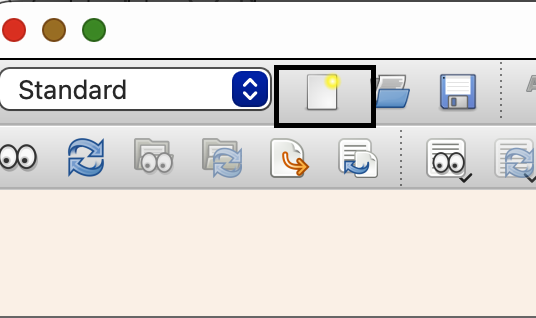
\includegraphics[keepaspectratio,alt={New Document}]{week2_lyx_new.png}}
\caption{New Document}
\end{figure}

\subsection{Select Document Class}\label{select-document-class}

Go to Document \(\rightarrow\) Settings.

\begin{figure}
\centering
\pandocbounded{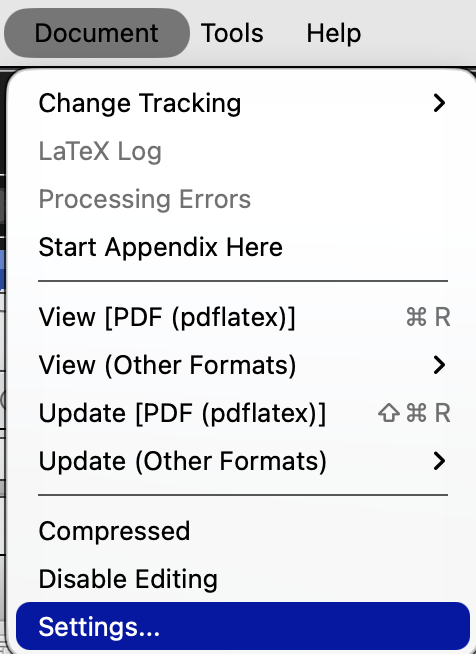
\includegraphics[keepaspectratio,alt={Lyx Document Settings}]{week2_lyx_docsetting.png}}
\caption{Lyx Document Settings}
\end{figure}

Make sure ``Article Standard Class'' is selected. This will provide the sections that we need for our document.

\begin{figure}
\centering
\pandocbounded{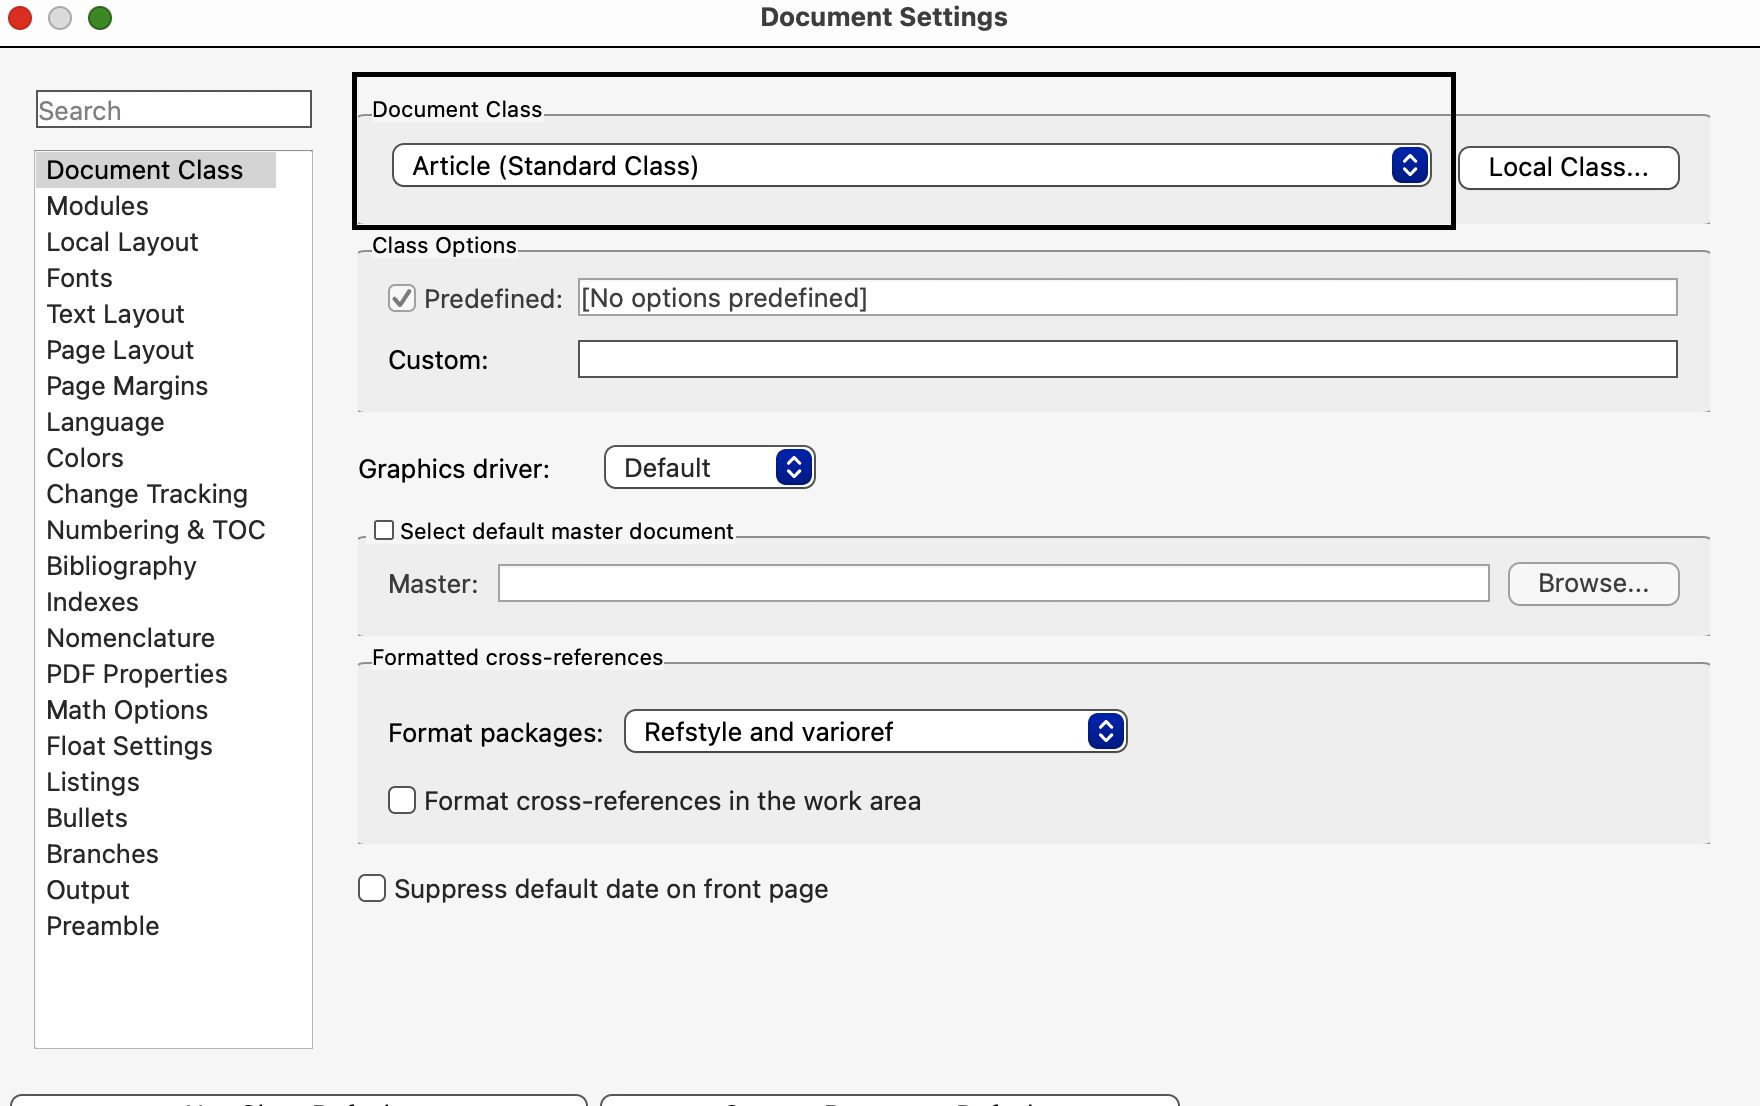
\includegraphics[keepaspectratio,alt={Article Standard Class}]{week2_lyx_docsetting2.png}}
\caption{Article Standard Class}
\end{figure}

Now go back to the main window and look to the upper left to see the Envionment window. It should should the word ``Standard''.

\begin{figure}
\centering
\pandocbounded{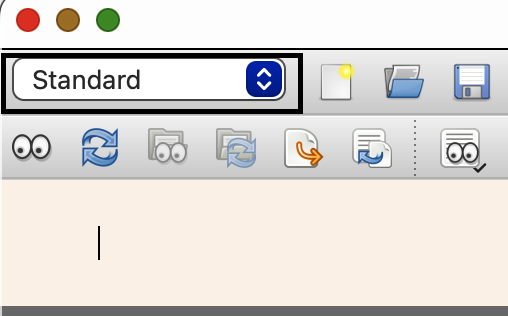
\includegraphics[keepaspectratio,alt={LyX Style Window}]{week2_lyx_styles2.png}}
\caption{LyX Style Window}
\end{figure}

\subsection{Sections}\label{sections}

After selecting ``Standard'' in the Environment window, go to ``Section'' under ``Sectioning''.

\begin{figure}
\centering
\pandocbounded{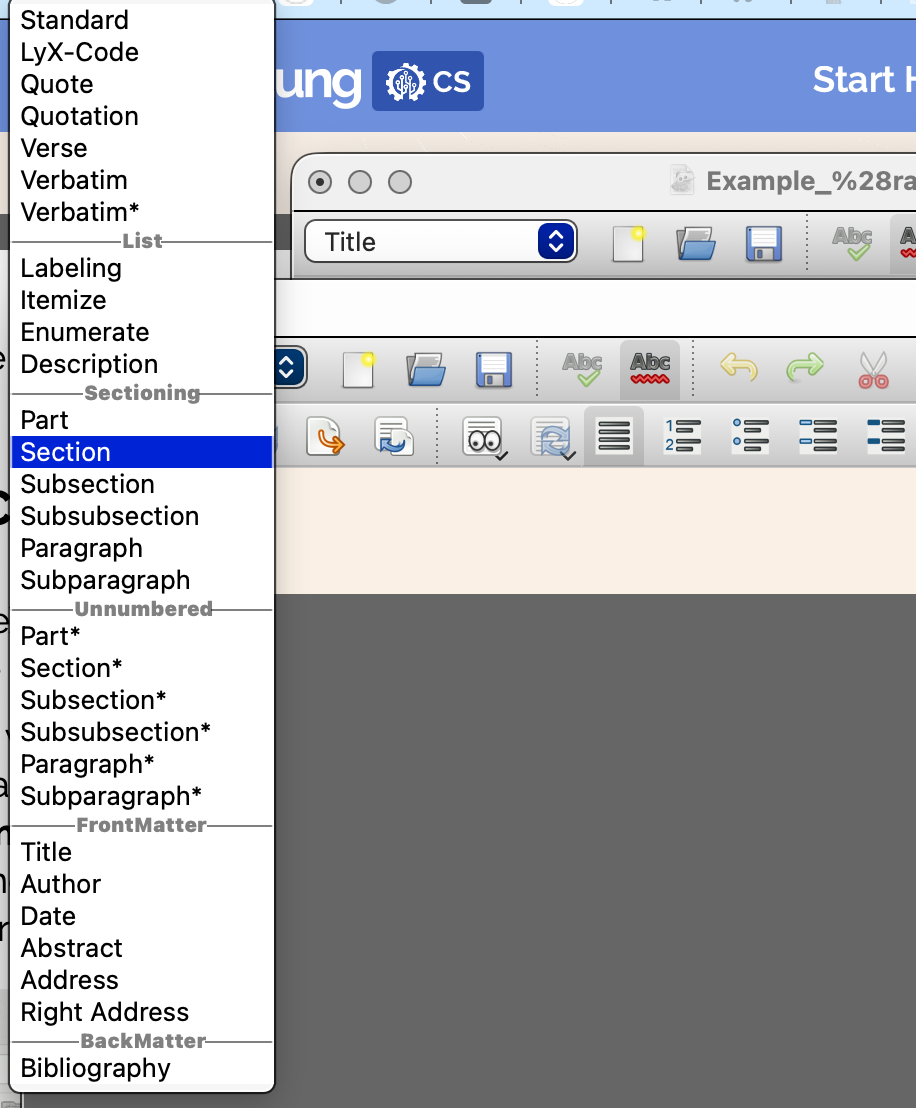
\includegraphics[keepaspectratio,alt={LyX Environment Window}]{week2_lyx_styles.png}}
\caption{LyX Environment Window}
\end{figure}

This will create a new section, which will look like this. Next, we can enter our section header, which will be ``Introduction'' for this example.

\begin{figure}
\centering
\pandocbounded{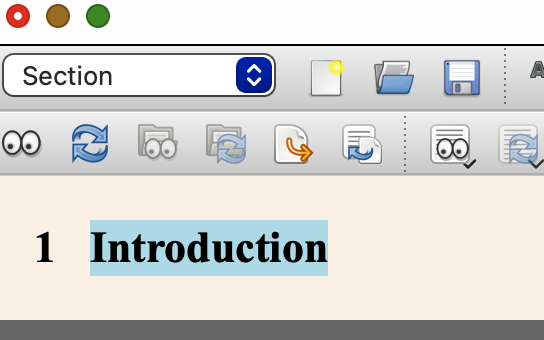
\includegraphics[keepaspectratio,alt={LyX Numbered Section 1}]{week2_lyx_section1.png}}
\caption{LyX Numbered Section 1}
\end{figure}

Next, press ``Enter'' and begin to type your introduction paragraph.

\begin{figure}
\centering
\pandocbounded{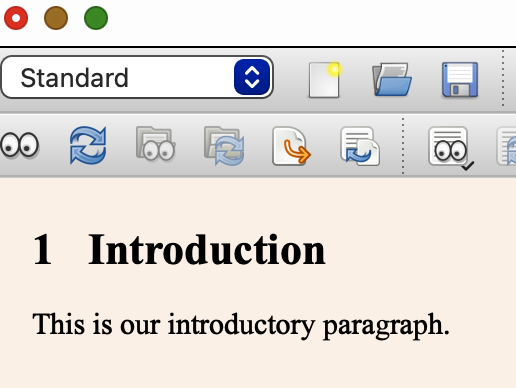
\includegraphics[keepaspectratio,alt={Introductory paragraph}]{week2_lyx_section1_1.png}}
\caption{Introductory paragraph}
\end{figure}

\subsection{Subsections}\label{subsections}

After your introduction paragraph(s), press enter for a new paragraph. You will notice that the new paragraph is indented. We will type the word ``Background'' for our first subsection. It will look like the following:

\begin{figure}
\centering
\pandocbounded{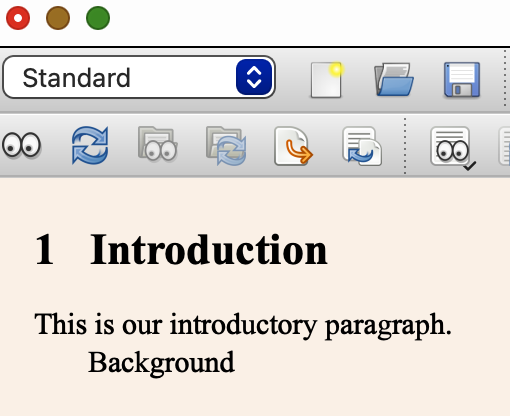
\includegraphics[keepaspectratio,alt={New paragraph indented}]{week2_lyx_section1_2.png}}
\caption{New paragraph indented}
\end{figure}

Now go back to the Environment window and select ``Subsection'' under ``Sectioning''.

\begin{figure}
\centering
\pandocbounded{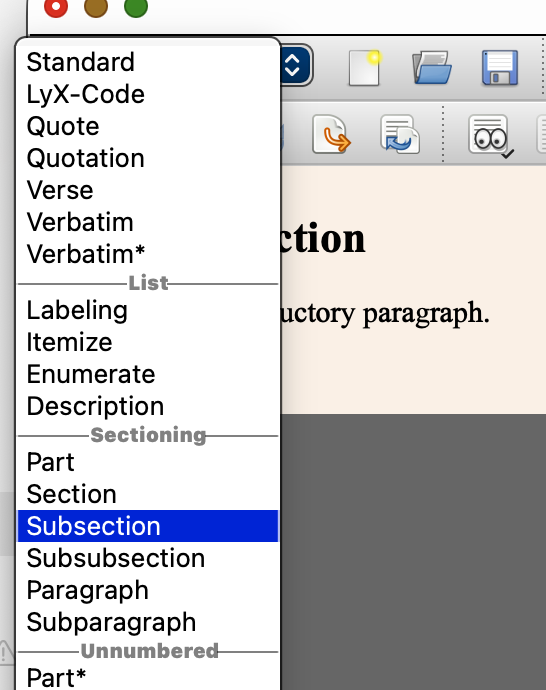
\includegraphics[keepaspectratio,alt={New Subsection Selection}]{week2_lyx_section1_3.png}}
\caption{New Subsection Selection}
\end{figure}

The result will be that ``Background'' becomes subsection 1.1.

\begin{figure}
\centering
\pandocbounded{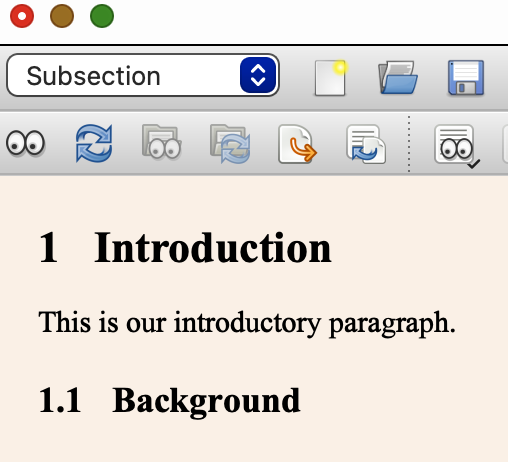
\includegraphics[keepaspectratio,alt={New Subsection Added}]{week2_lyx_section1_4.png}}
\caption{New Subsection Added}
\end{figure}

We can do this several subsections. We will create ``Theory'' and ``Literature Review'' subsections.

\begin{figure}
\centering
\pandocbounded{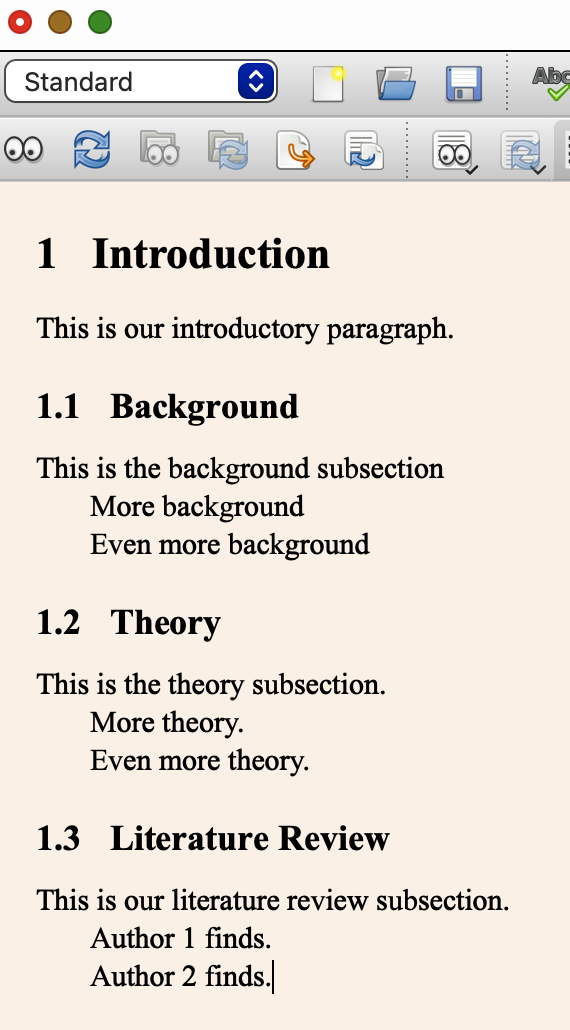
\includegraphics[keepaspectratio,alt={Additional subsections}]{week2_lyx_section1_5.png}}
\caption{Additional subsections}
\end{figure}

\subsection{Preview our work}\label{preview-our-work}

Now that we have created our first section. Let's preview what our pdf will look like. Click the preview button to see the preview.

\begin{figure}
\centering
\pandocbounded{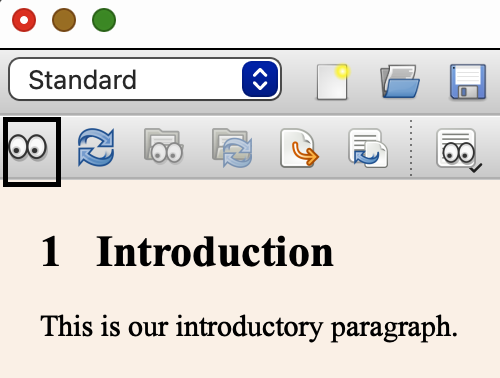
\includegraphics[keepaspectratio,alt={Preview your work}]{week2_lyx_preview.png}}
\caption{Preview your work}
\end{figure}

\subsection{Title, Author, and Abstract}\label{title-author-and-abstract}

Let's add a title to our article. Go to the first line and enter your title of the article. In this example, we will call the article ``Econ 643 LyX Example''.

\begin{figure}
\centering
\pandocbounded{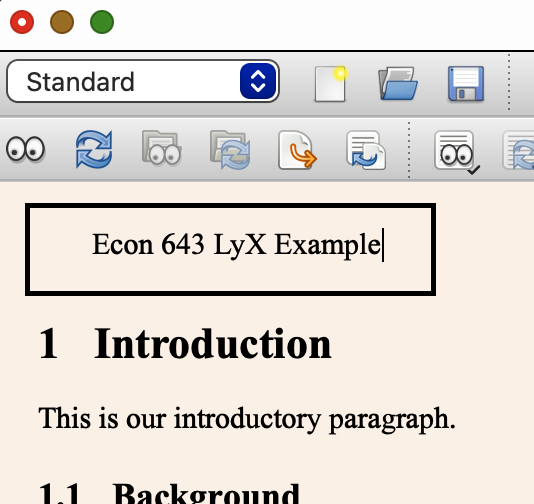
\includegraphics[keepaspectratio,alt={Add a Title}]{week2_lyx_title1.png}}
\caption{Add a Title}
\end{figure}

Go back to the Environment window and select ``Title'' under ``Front Matter''.

\begin{figure}
\centering
\pandocbounded{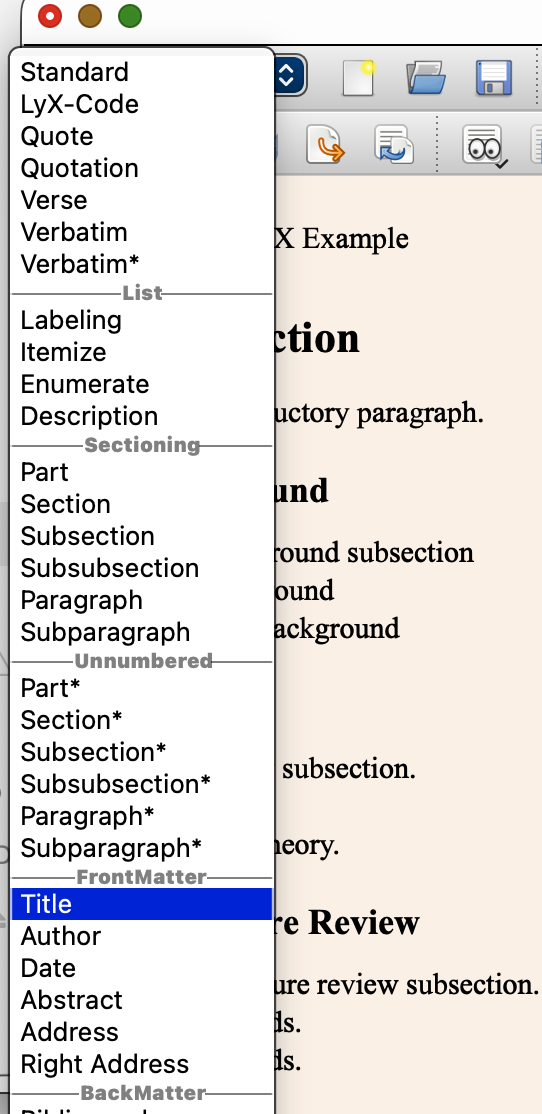
\includegraphics[keepaspectratio,alt={Title Option}]{week2_lyx_title2.png}}
\caption{Title Option}
\end{figure}

Select ``Title'' and your title will become a title for your article.

\begin{figure}
\centering
\pandocbounded{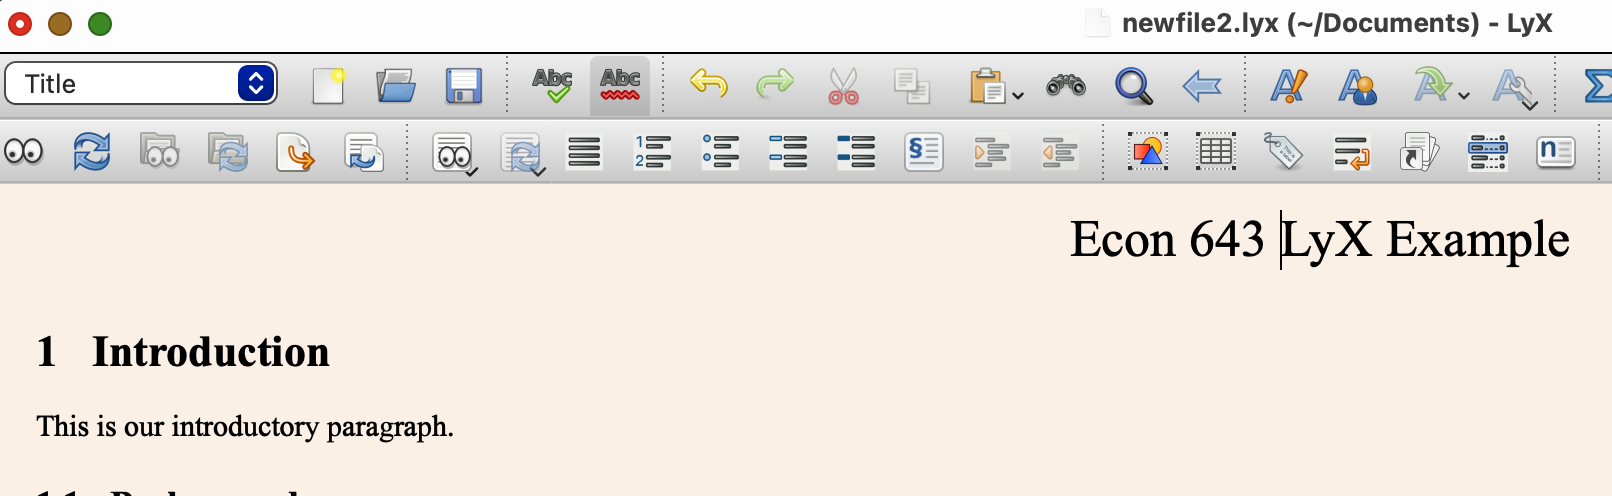
\includegraphics[keepaspectratio,alt={New Title}]{week2_lyx_title3.png}}
\caption{New Title}
\end{figure}

\subsection{Add an author}\label{add-an-author}

Under your title, add your name.

Next select ``Author'' under the ``Front Matter'' section of the Environment window.

\subsection{Table of Contents}\label{table-of-contents}

We can add a table of contents (optional). As long as we are using sectioning, a table of contents will automatically generate once we select

\subsection{Mathematical Equations}\label{mathematical-equations}

We can click the following button to insert a mathematical equation into a LyX document.

\begin{figure}
\centering
\pandocbounded{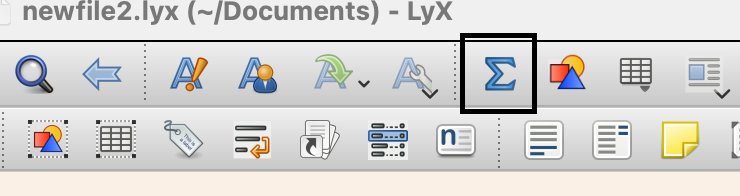
\includegraphics[keepaspectratio,alt={Mathematical Equation in LyX}]{week2_matheq.png}}
\caption{Mathematical Equation in LyX}
\end{figure}

\subsection{Insert LaTex Results}\label{insert-latex-results}

We can export our LaTex code that is produced from Stata with the \emph{estout} commands. When you preview the document, you will notice that there is LaTex code that automatically labels the table number.

To insert a place to insert the LaTex output from Stata, click Insert \(\rightarrow\) Tex Code.

\begin{figure}
\centering
\pandocbounded{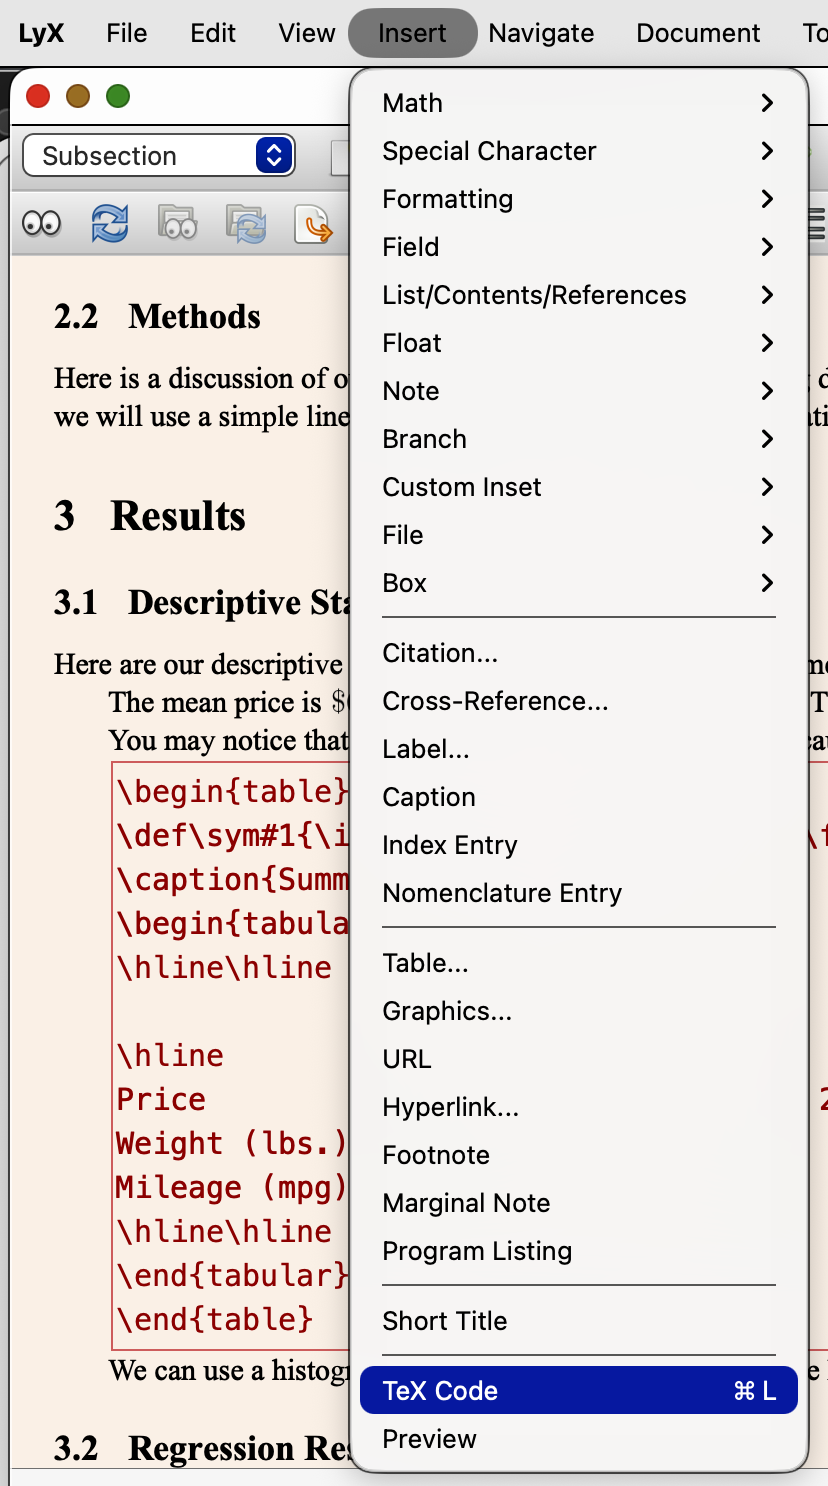
\includegraphics[keepaspectratio,alt={Insert Function}]{week2_lyx_insert1.png}}
\caption{Insert Function}
\end{figure}

Now you will see a new box in your Lyx Document.

\begin{figure}
\centering
\pandocbounded{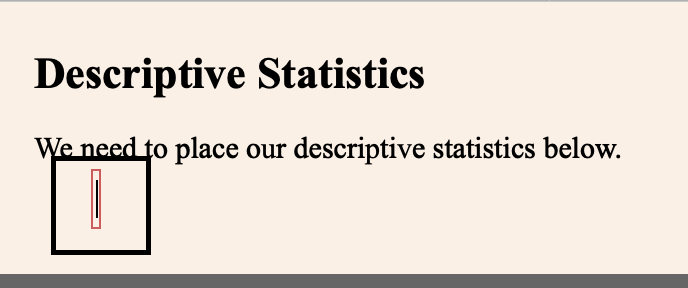
\includegraphics[keepaspectratio,alt={LaTex insert box}]{week2_lyx_insert2.png}}
\caption{LaTex insert box}
\end{figure}

Next paste your LaTex code output from Stata into Lyx with right-click and Paste.

\begin{figure}
\centering
\pandocbounded{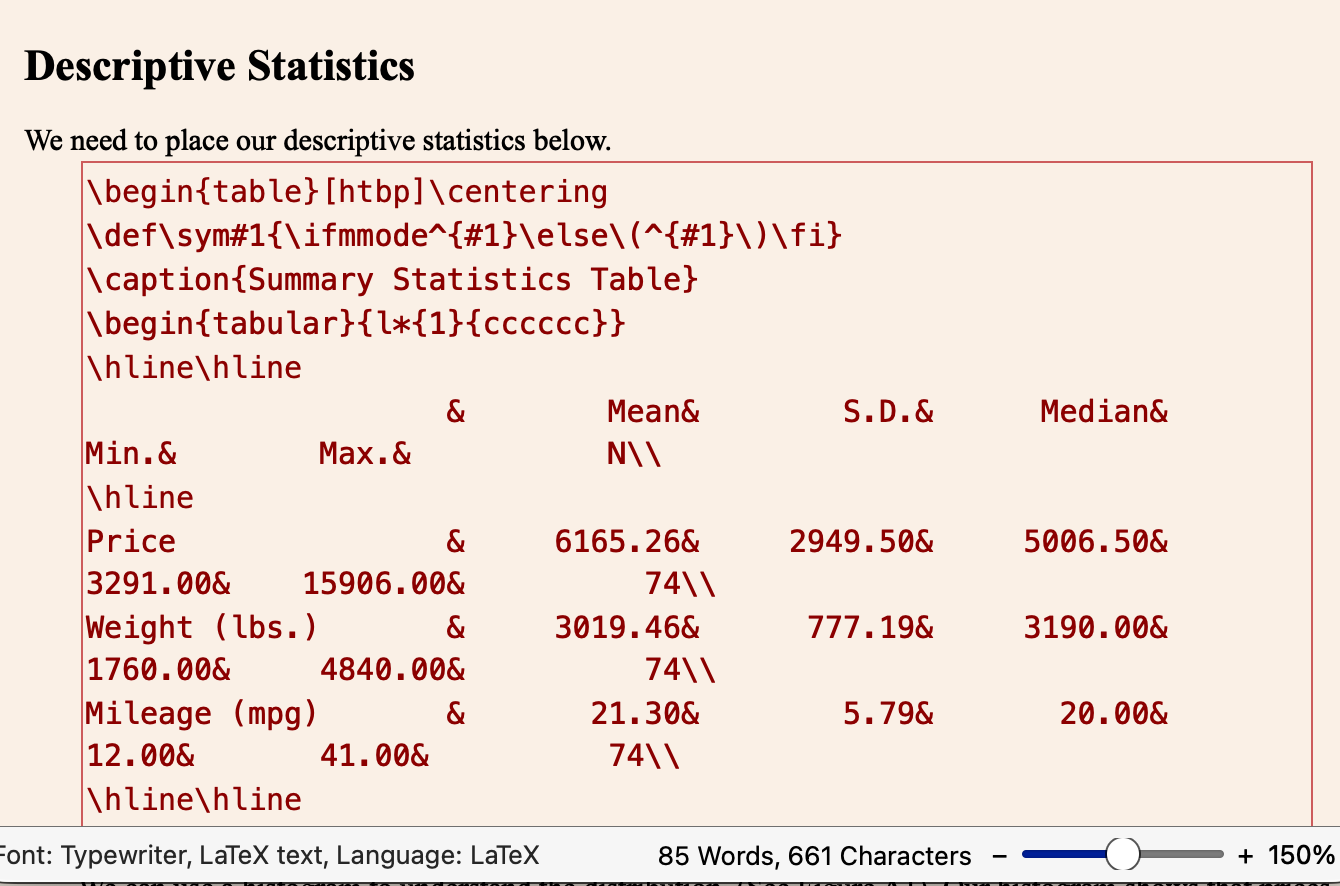
\includegraphics[keepaspectratio,alt={LaTex Right-Click Paste}]{week2_lyx_insert3.png}}
\caption{LaTex Right-Click Paste}
\end{figure}

We will discuss \emph{estout} in the next chapter.

\subsection{Insert Figure}\label{insert-figure}

Our final tutorial will cover inserting graphs from Stata. We will cover exporting graphs from Stata a bit later.

We need to export our Stata histogram that we created. We will save it as a ``.png'' file.

\begin{figure}
\centering
\pandocbounded{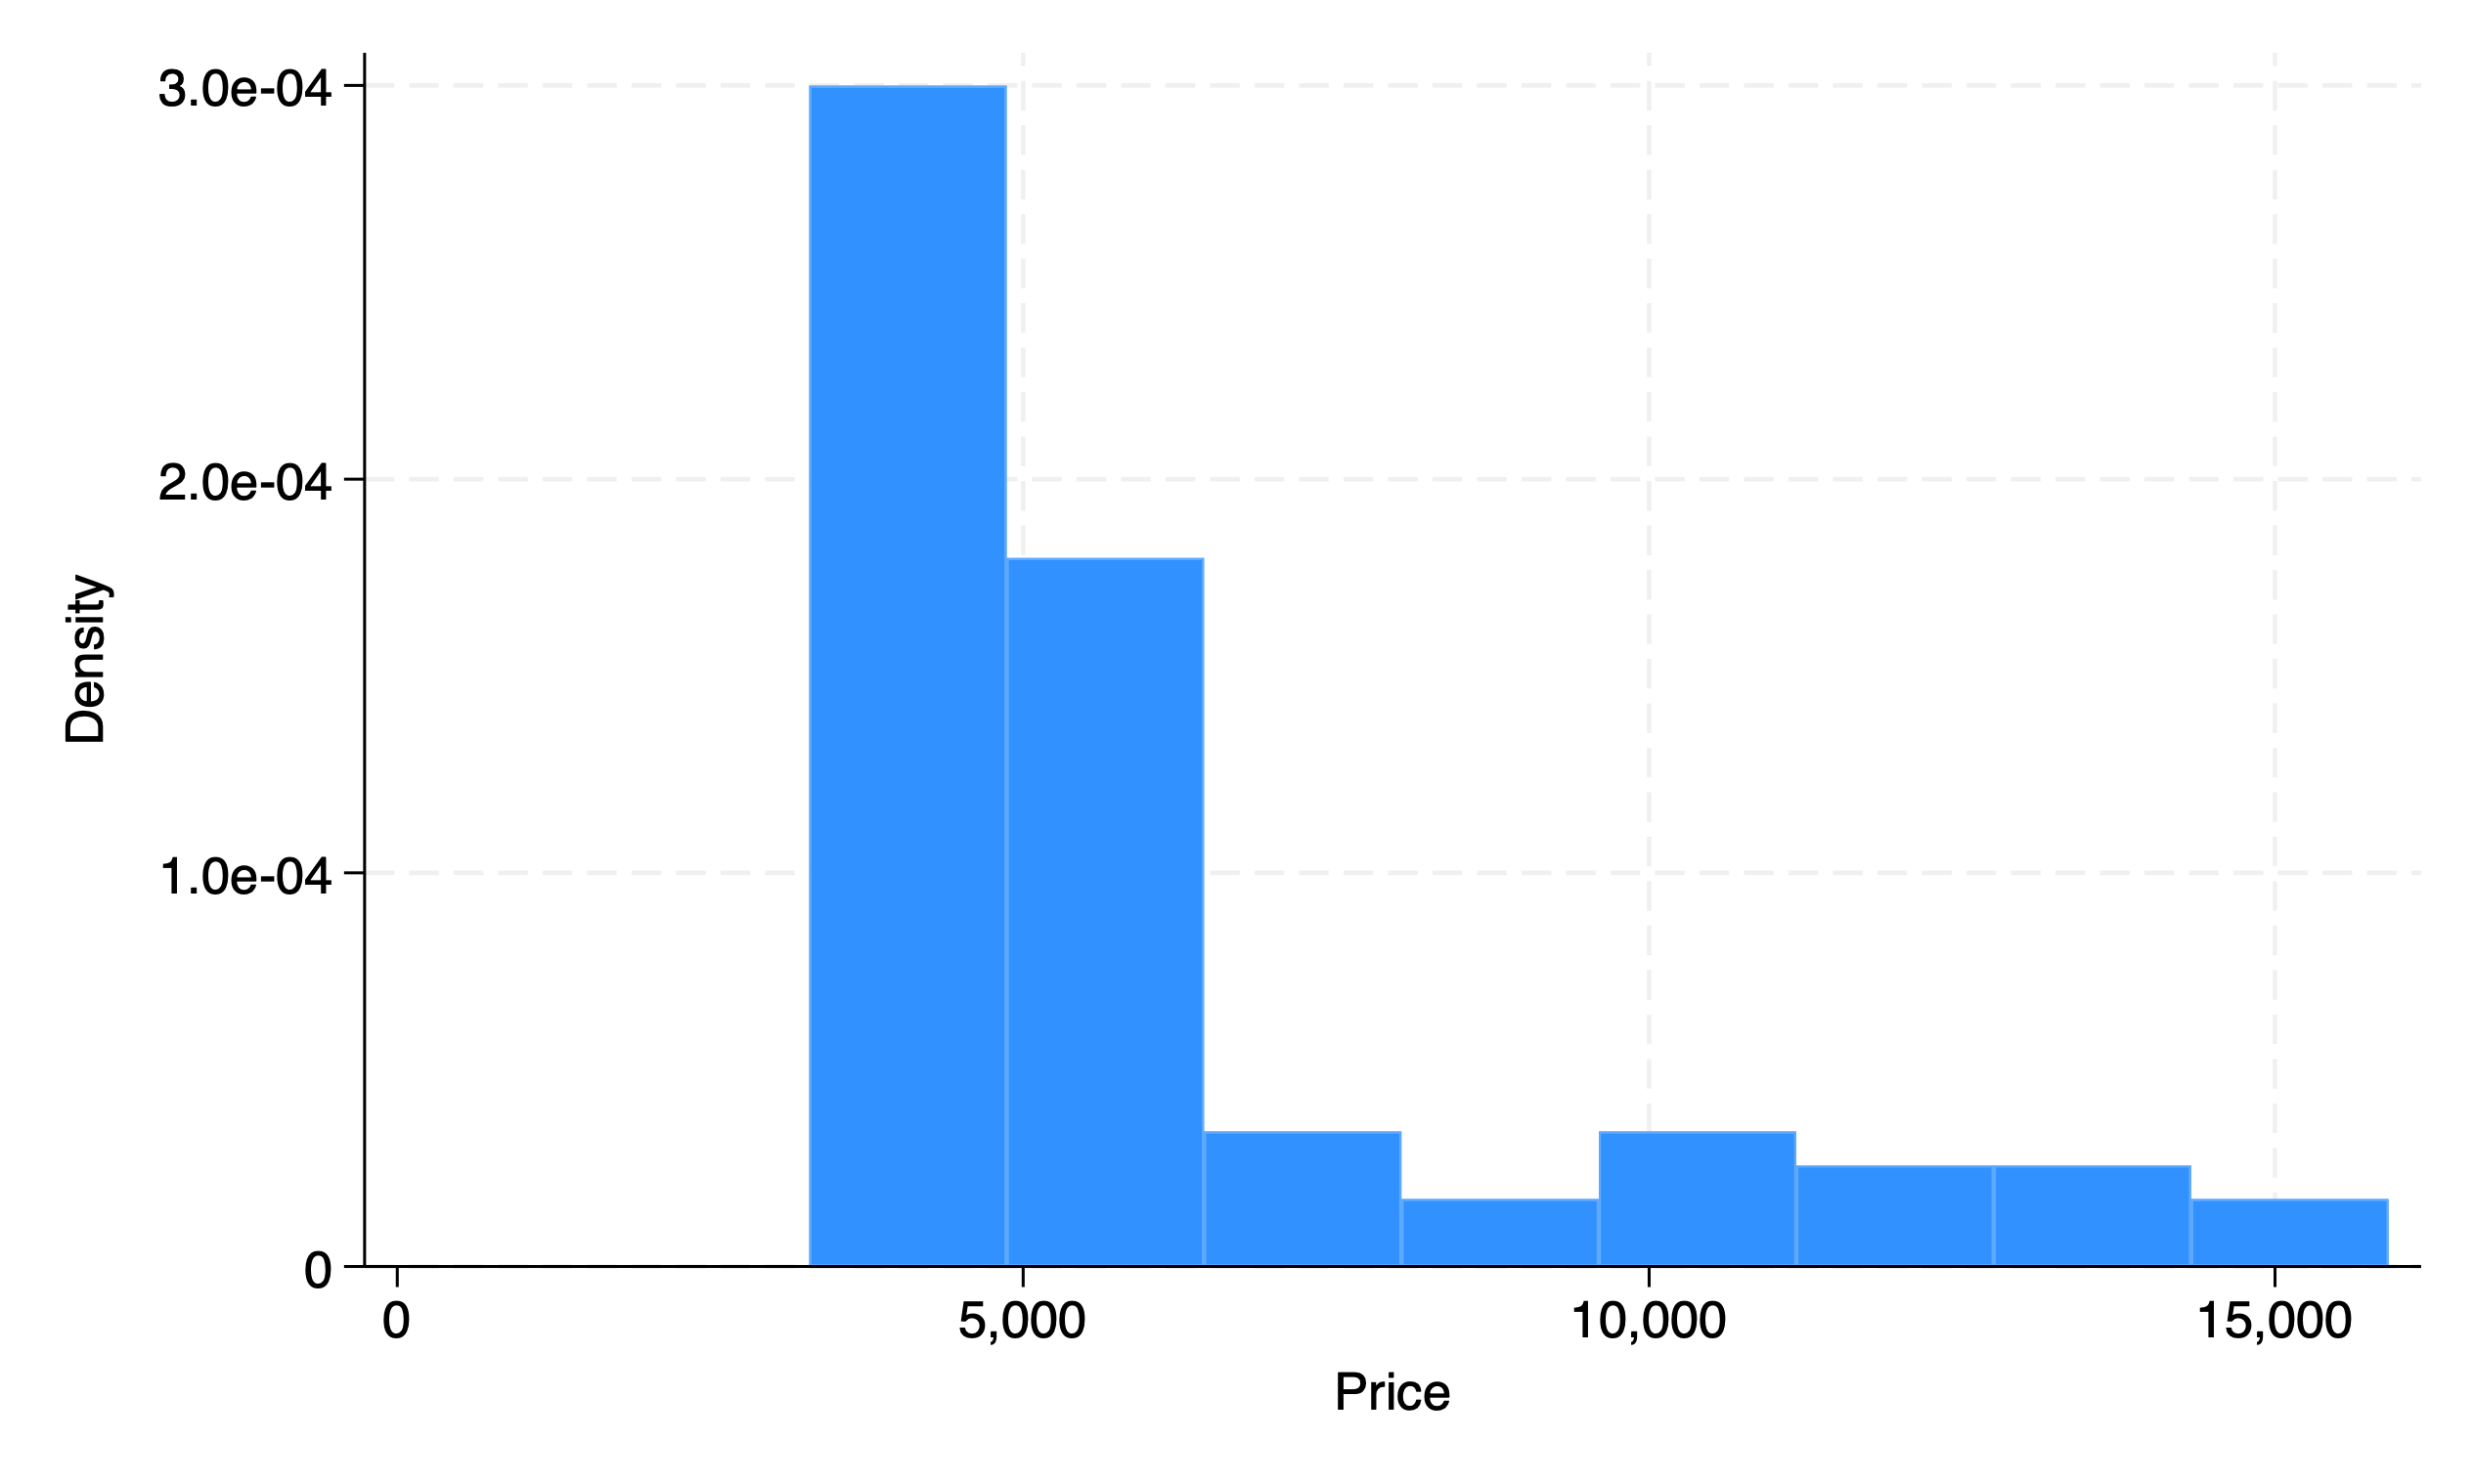
\includegraphics[keepaspectratio,alt={Histogram we want to insert}]{week2_lyx_hist.png}}
\caption{Histogram we want to insert}
\end{figure}

Go to Insert \(\rightarrow\) Float \(\rightarrow\) Figure.

\begin{figure}
\centering
\pandocbounded{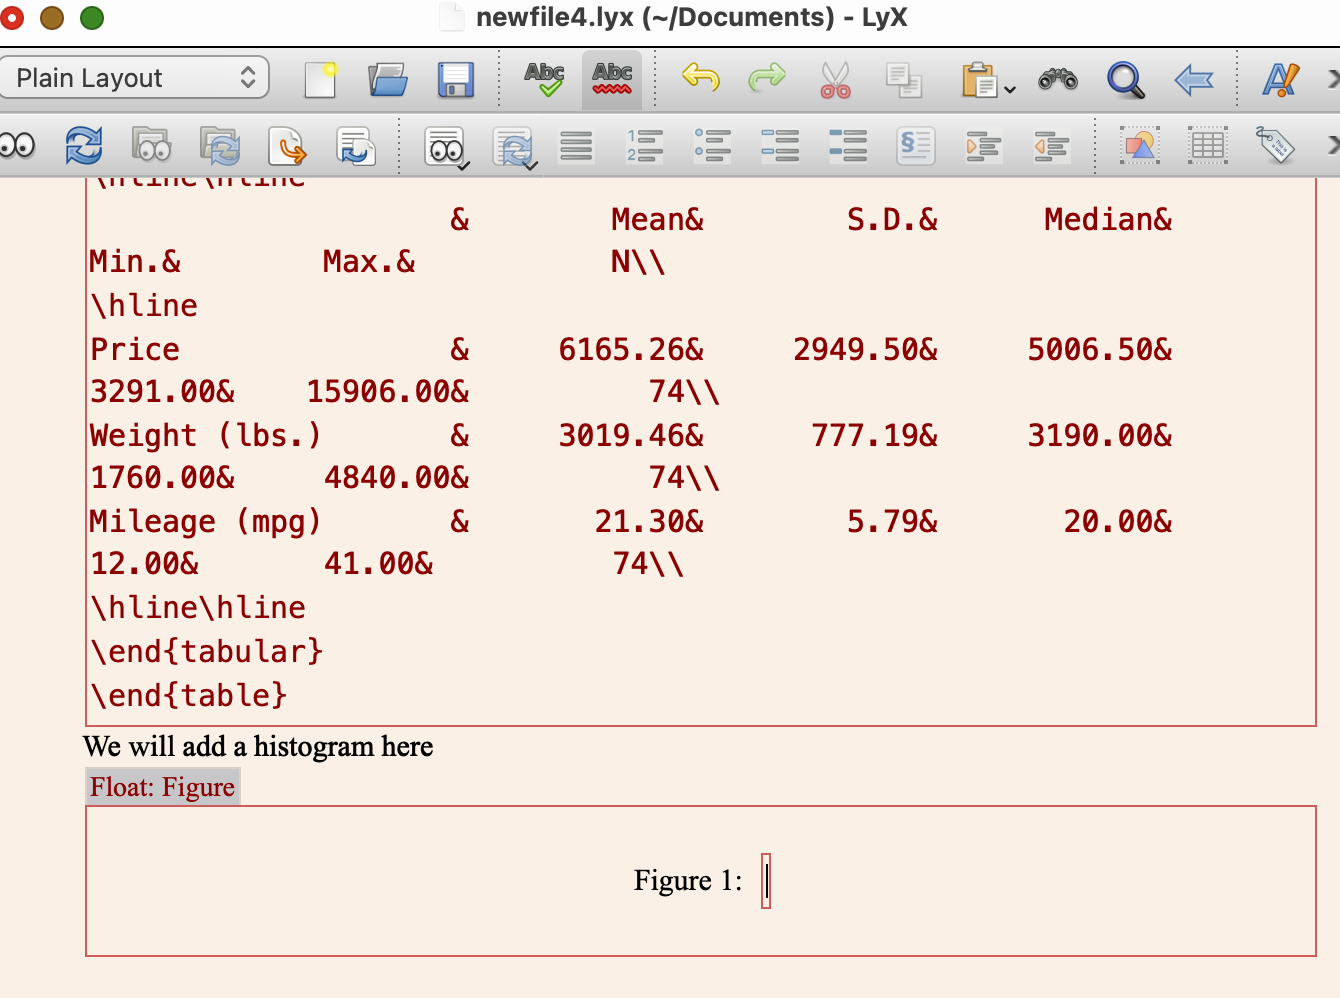
\includegraphics[keepaspectratio,alt={Insert Figure}]{week2_lyx_hist3.png}}
\caption{Insert Figure}
\end{figure}

Now enter a title for the figure. We will use ``Histogram of Automobile Price''.

\begin{figure}
\centering
\pandocbounded{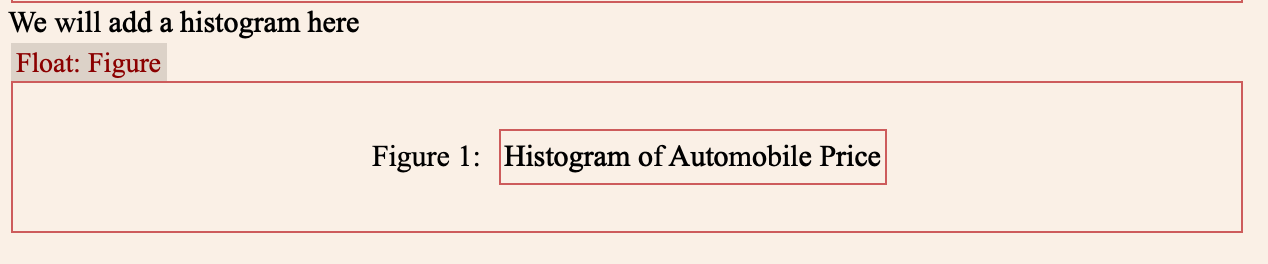
\includegraphics[keepaspectratio,alt={Figure Title}]{week2_lyx_hist4.png}}
\caption{Figure Title}
\end{figure}

Next, we need to insert the histogram from Stata above the Figure 1: box but below Float Figure. Go to Insert \(\rightarrow\) Graphics.

\begin{figure}
\centering
\pandocbounded{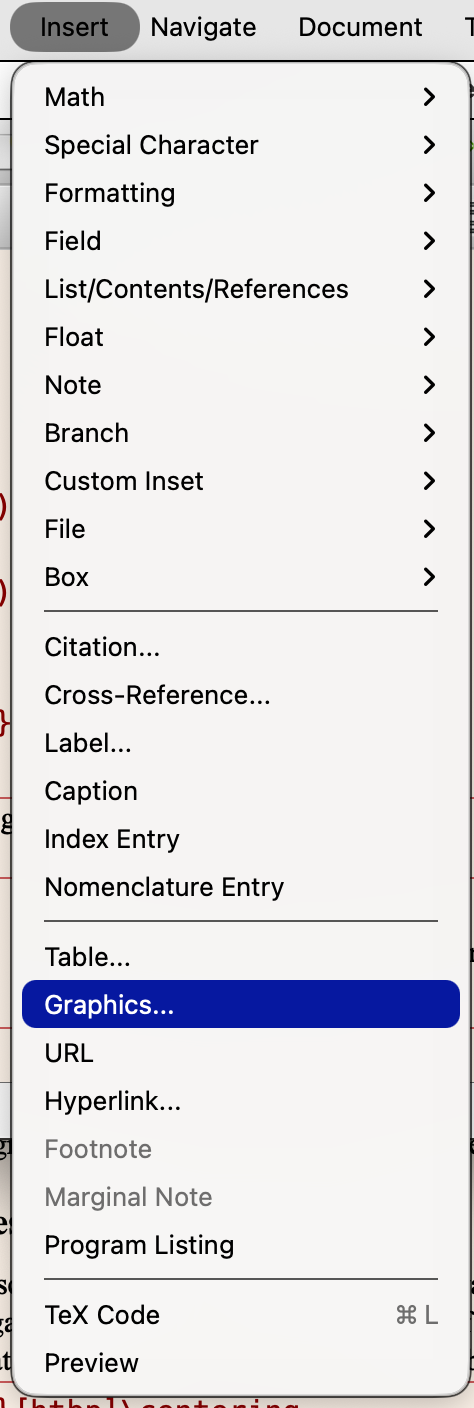
\includegraphics[keepaspectratio,alt={Insert Graphics}]{week2_lyx_hist5.png}}
\caption{Insert Graphics}
\end{figure}

In the Graphics window, click browse and find your histogram ``.png'' file. Next, select ``set width'' and choose the size of your choice. Next, select ``Column Width \%'' from the drop down menu next to ``set width''. Click ``OK''.

\begin{figure}
\centering
\pandocbounded{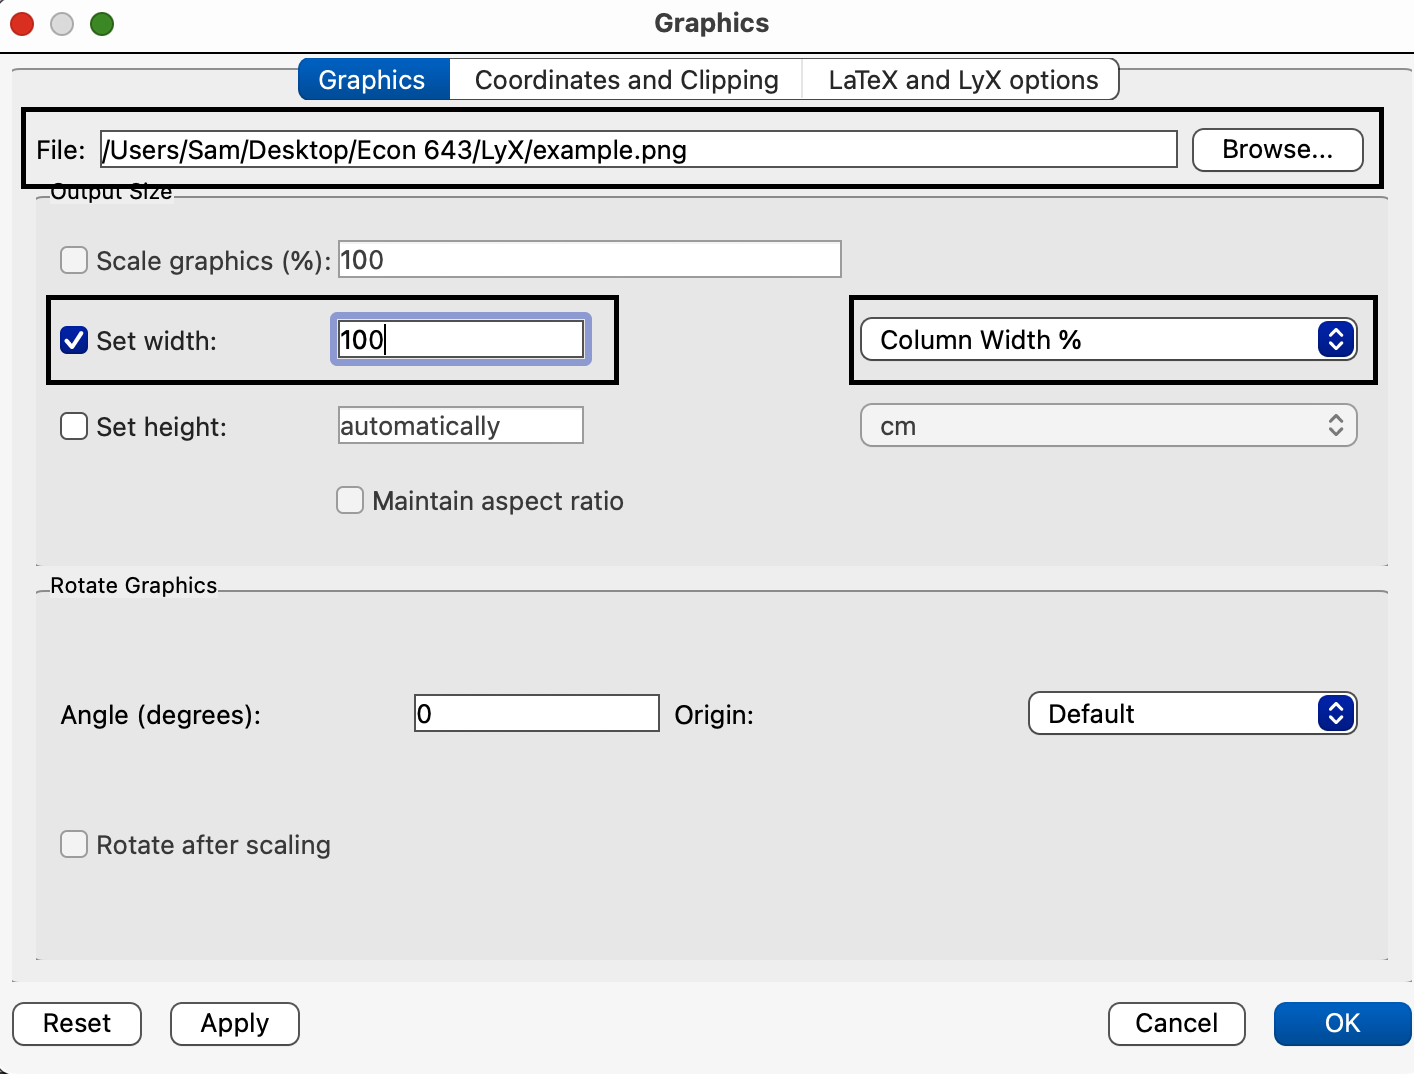
\includegraphics[keepaspectratio,alt={Graphics Window}]{week2_lyx_hist6.png}}
\caption{Graphics Window}
\end{figure}

Your histogram will be inserted, but it may look funny.

\begin{figure}
\centering
\pandocbounded{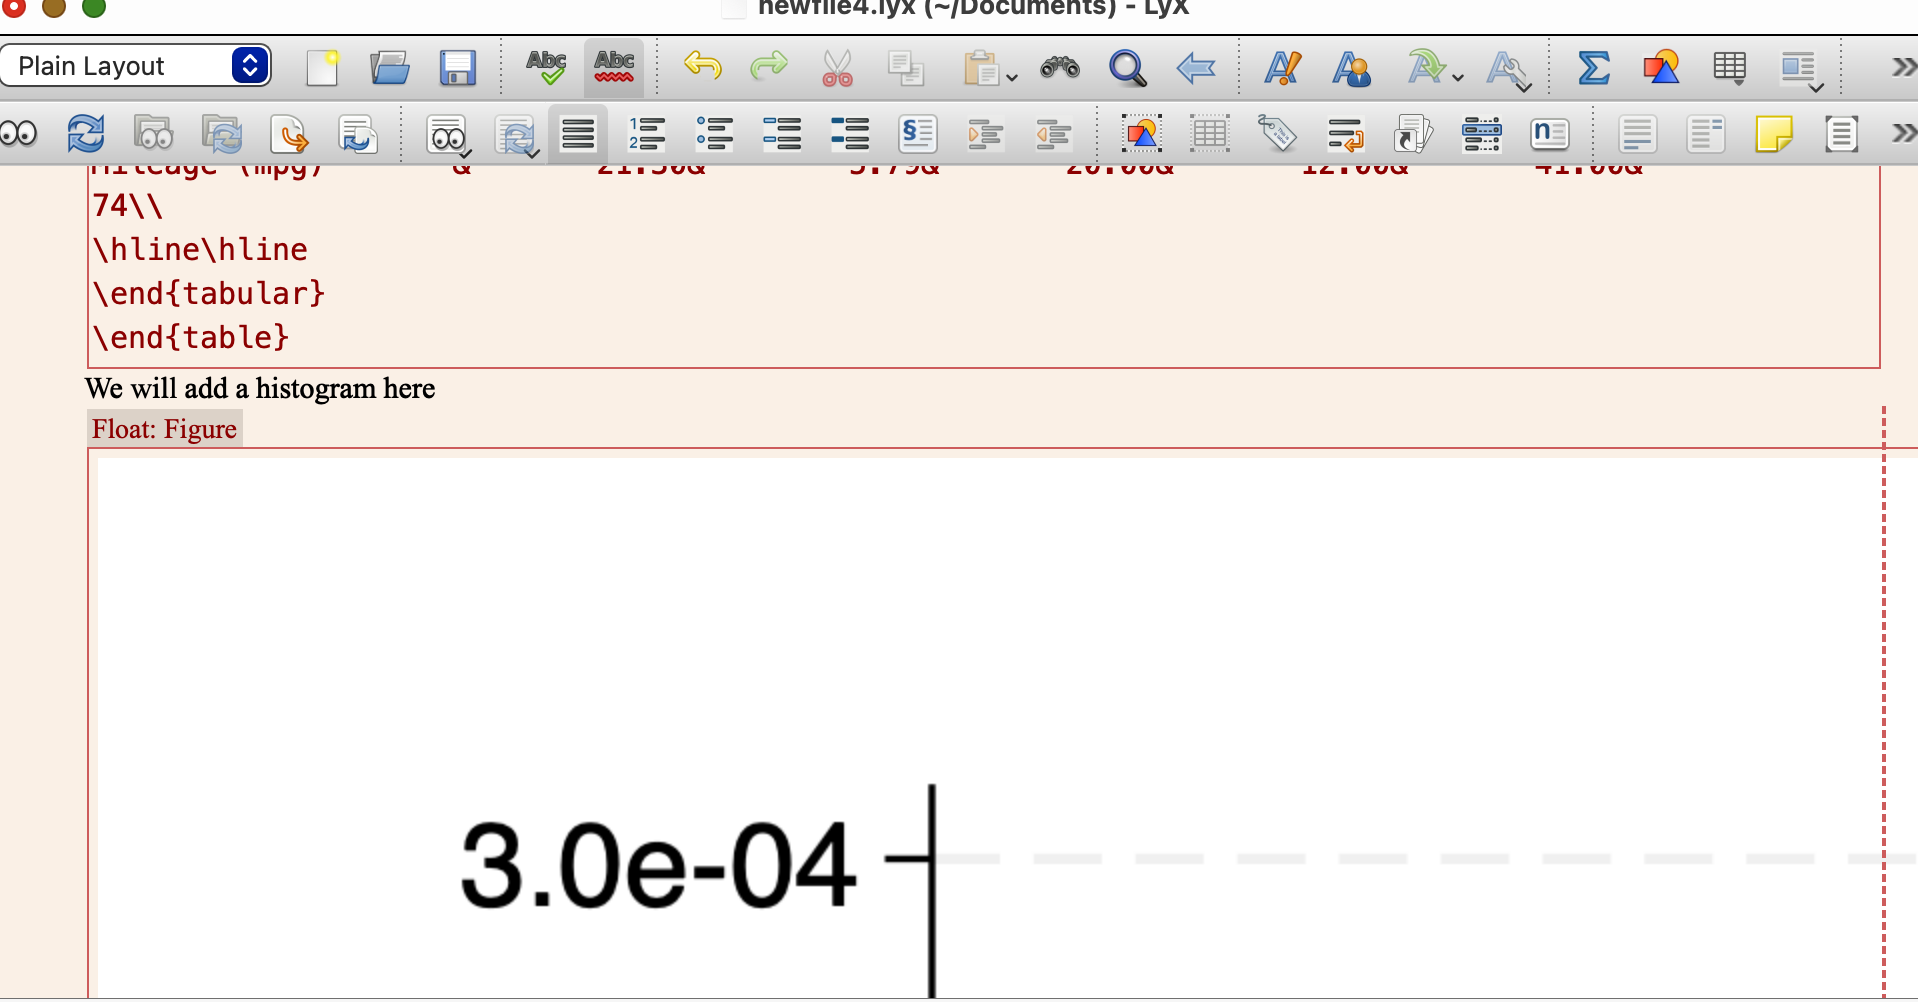
\includegraphics[keepaspectratio,alt={Inserted Histogram}]{week2_lyx_hist7.png}}
\caption{Inserted Histogram}
\end{figure}

Click on preview to see how well the histogram was inserted. You may need to play around with the settings. I have the size of the Stata graph window makes the graphic file larger.

\begin{figure}
\centering
\pandocbounded{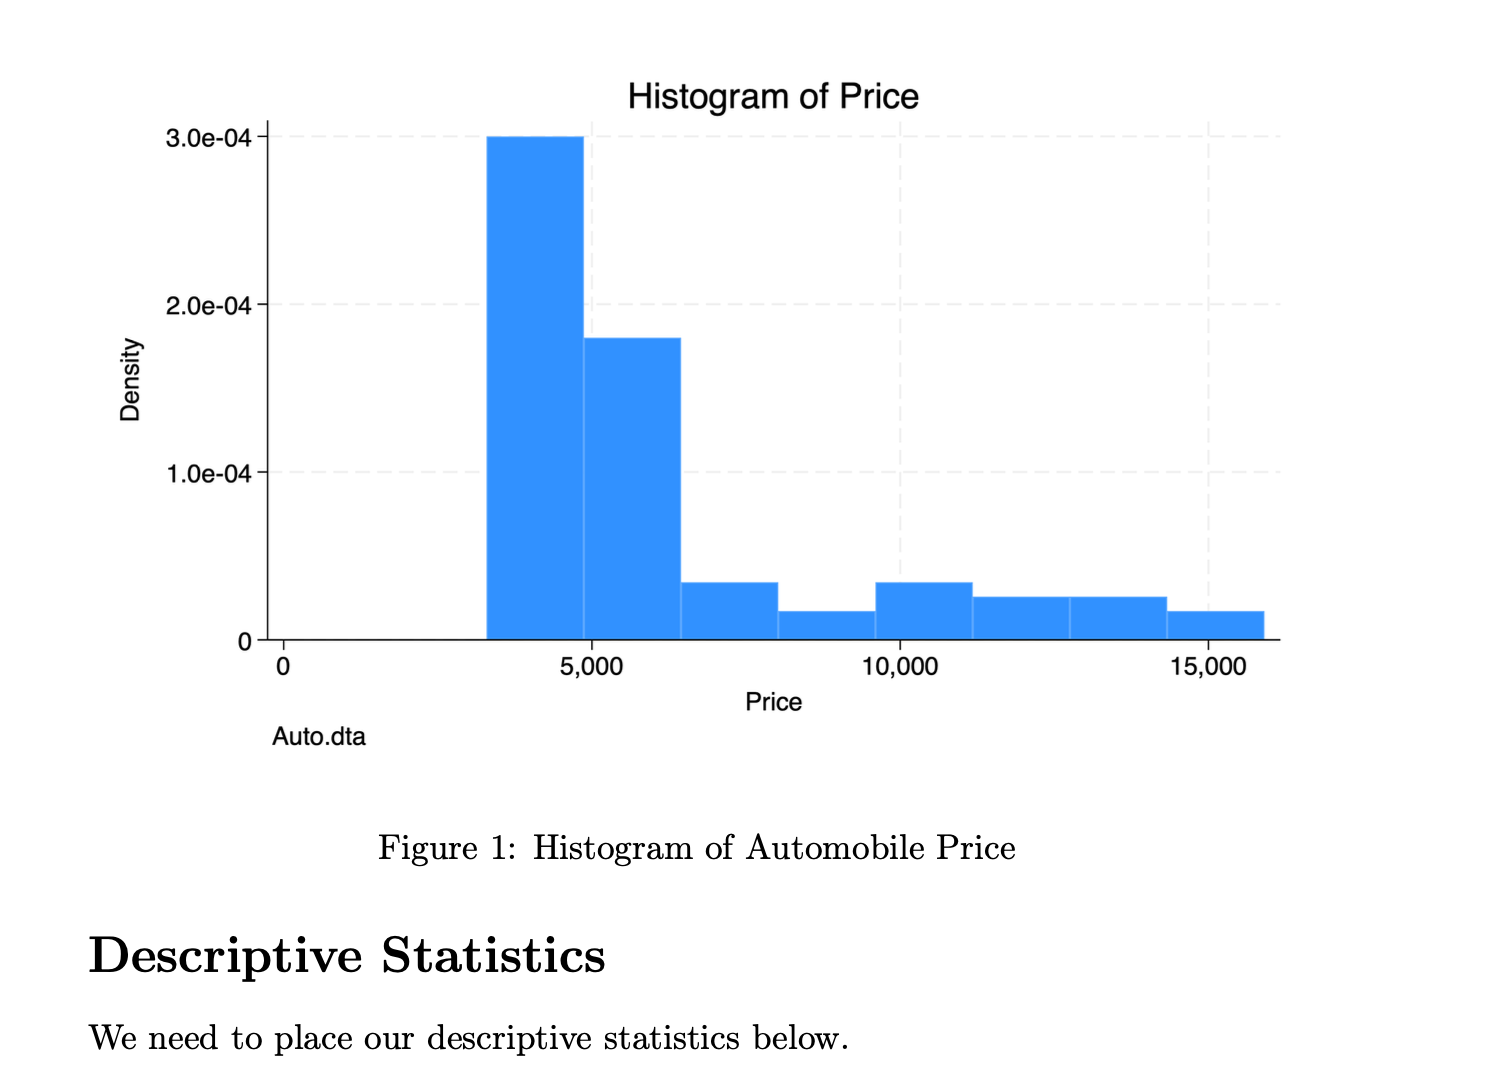
\includegraphics[keepaspectratio,alt={Inserted Histogram PDF}]{week2_lyx_hist8.png}}
\caption{Inserted Histogram PDF}
\end{figure}

\section{Export Your LaTex file into PDF}\label{export-your-latex-file-into-pdf}

Go to File \(\rightarrow\) Export \(\rightarrow\) Export As. Select the location of the folder you want to store the file. Next, enter the name of the file and select ``PDF (pdflatex) (*.pdf)``.

\begin{figure}
\centering
\pandocbounded{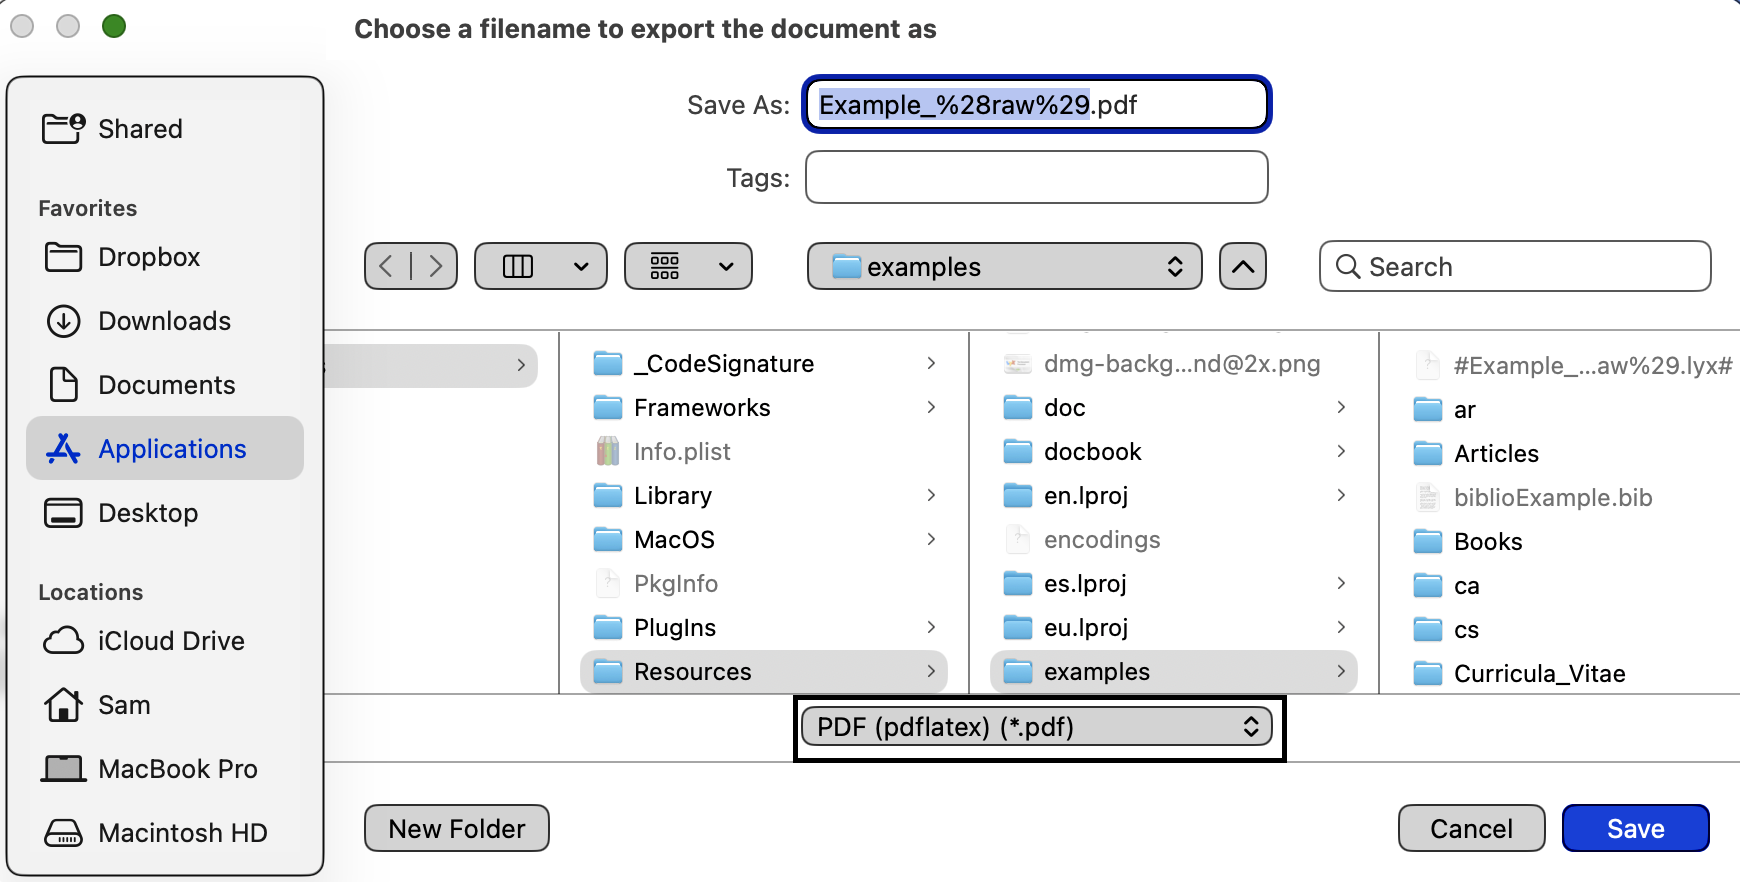
\includegraphics[keepaspectratio,alt={Export As in LyX}]{week2_lyx_exportas.png}}
\caption{Export As in LyX}
\end{figure}

\chapter{Introduction to LaTex}\label{introduction-to-latex}

I will provide a crash course on how to use LaTex to create mathematical equations. Kemp, et al.~(2016) discuss how LaTeX is the ``industry standard'' typesetting system for writing mathematics. LaTeX is more flexible than standard word processors, such as MSWord), produces vastly better-looking results.

Learning how to create mathematical equations with LaTex will help you with your homework and projects through the empirical sequence.

With LaTex, we can turn y=bx\^{}2+c into \[ y=\beta x^2 + c \]

If you want a mean, you don't have to type mu or average. Just use LaTex by entering ``\textbackslash~mu'' which results in \(\mu\). Do you want to expected value of x? You can just use E(x), but it looks better with LaTex with \(E(x)\).

\section{How to use mathematical symbols}\label{how-to-use-mathematical-symbols}

We typicall use the ``\textbackslash" to initate a mathemetical symbol. We can use''\^{}'' for superscripts and ``\emph{'' for subscripts. For example, we can type \textbackslash~sum\^{}N}\{i=1\} x\_\{i\} and it will become \[ \sum^N_{i=1} x_{i} \]

You may have noticed that the subscripts had \{\} brackets. When we want to include an equation in the subscript or subscript, we need to include \{\} brackets, such as x\^{}\{2a+3b\}. This will result in \(x^{2a+3b}\)

\section{Overview of mathematical symbols}\label{overview-of-mathematical-symbols}

I think the following is a helpful reference guide for mathematical symbols in LaTex

\pandocbounded{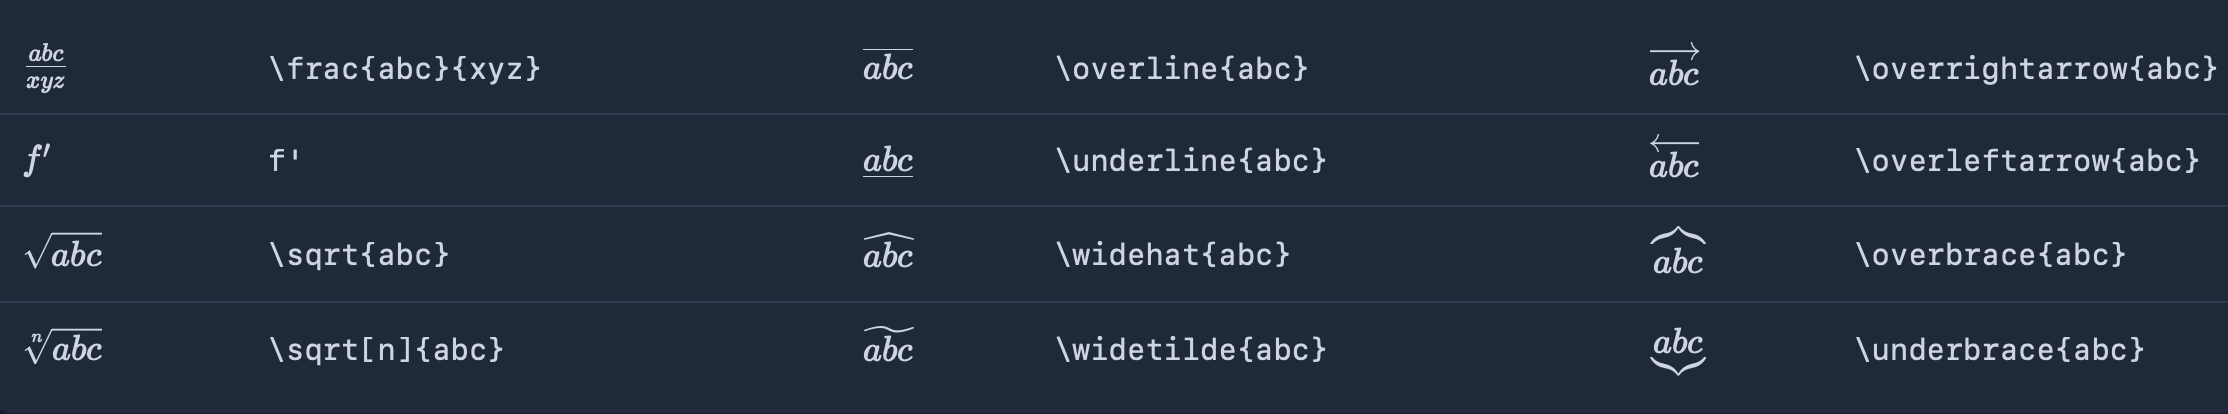
\includegraphics[keepaspectratio,alt={Mathematical expressions}]{week2_latex2.png}}
Source: \url{https://quickref.me/latex.html}

\section{Greek letters}\label{greek-letters}

\pandocbounded{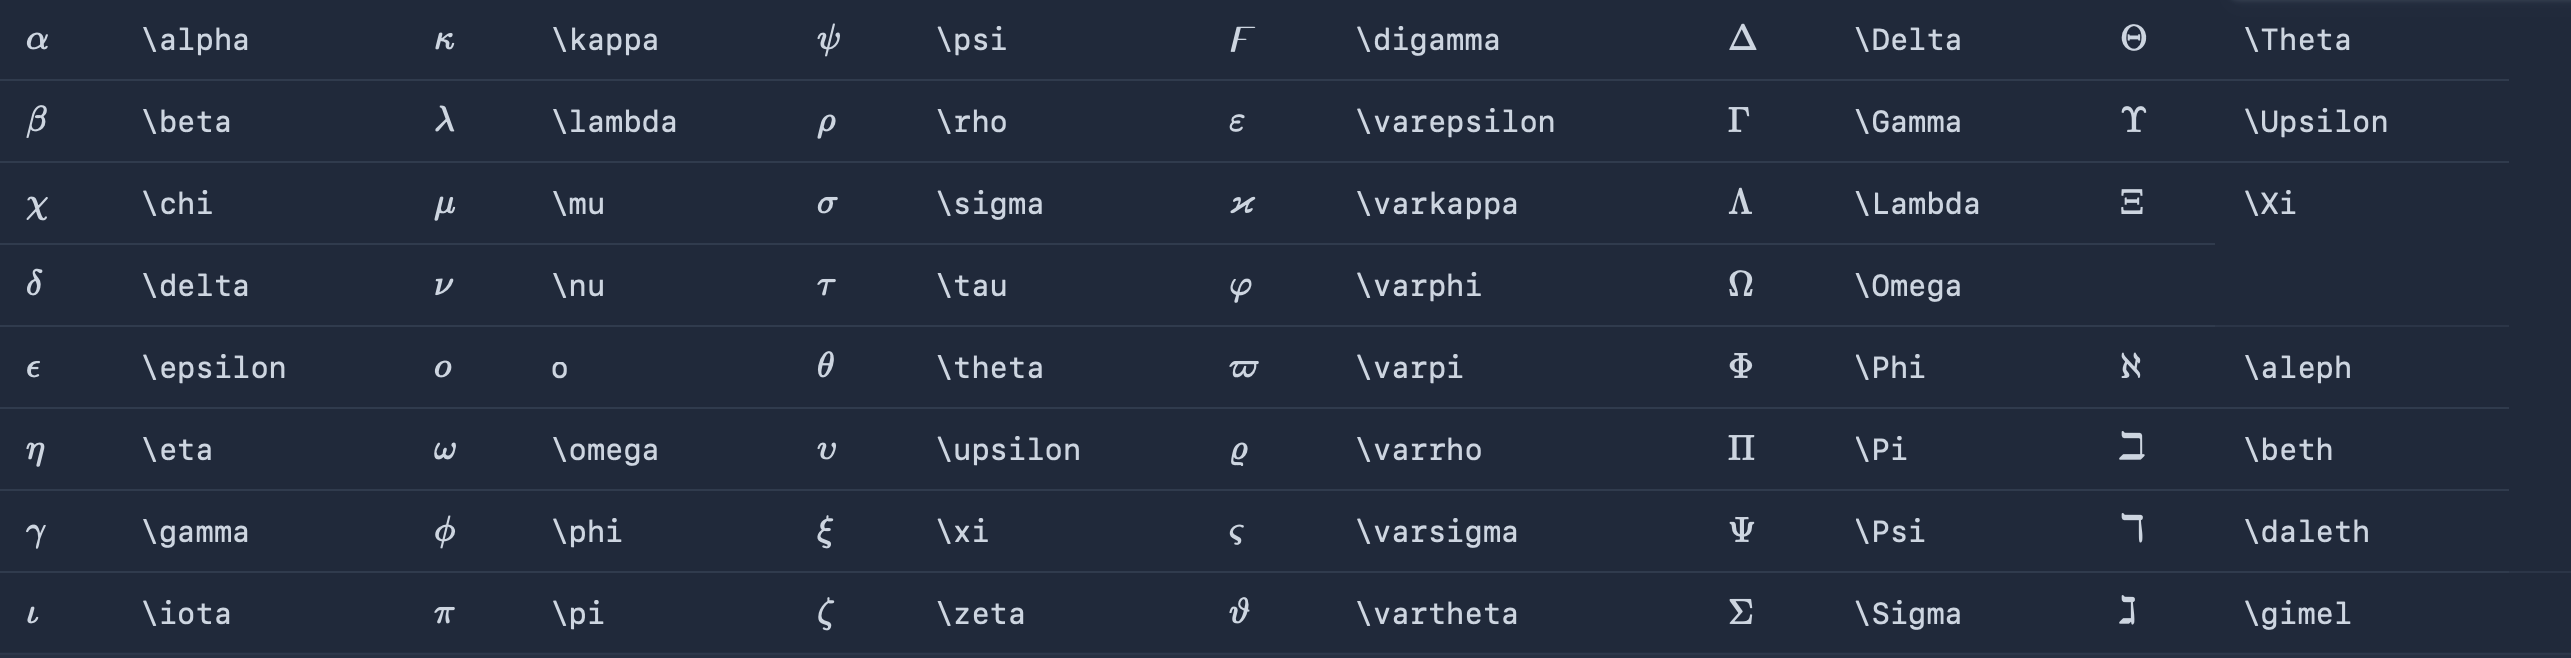
\includegraphics[keepaspectratio,alt={Greek letters Overview}]{week2_latex1.png}}
Source: \url{https://quickref.me/latex.html}

\section{Accents and Braces}\label{accents-and-braces}

\pandocbounded{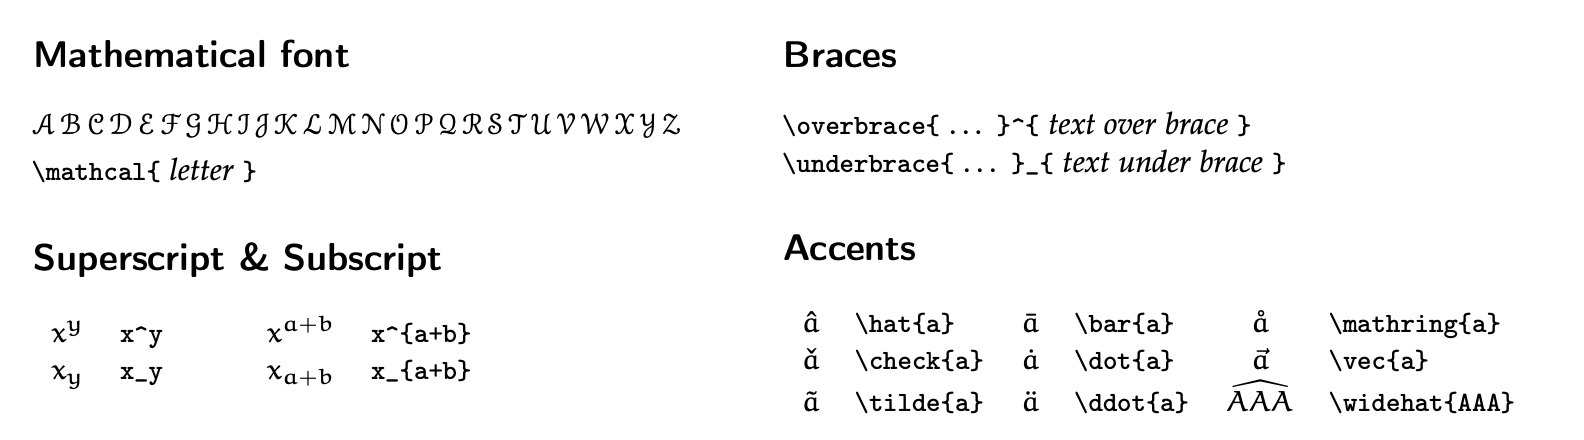
\includegraphics[keepaspectratio,alt={Accents, Scripts, and Braces Overview}]{week2_latex_accents.png}}
Source: \url{https://www.tilburgsciencehub.com/topics/research-skills/templates-dynamic-content/templates/amsmath-latex-cheatsheet/}

\section{Binary Relations and Operators}\label{binary-relations-and-operators}

\begin{figure}
\centering
\pandocbounded{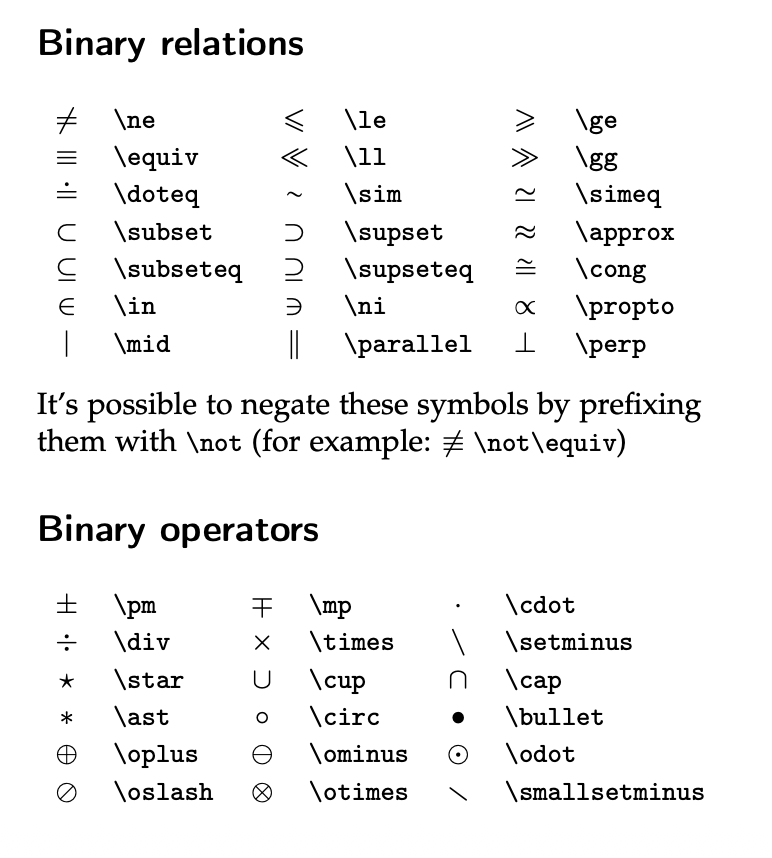
\includegraphics[keepaspectratio,alt={Binary Relations and Operators}]{week2_latex_binary.png}}
\caption{Binary Relations and Operators}
\end{figure}

Source: \url{https://www.tilburgsciencehub.com/topics/research-skills/templates-dynamic-content/templates/amsmath-latex-cheatsheet/}

\chapter{Incorporating LaTex output from Stata}\label{incorporating-latex-output-from-stata}

\section{Table commands}\label{table-commands}

\emph{Table} command is provides a basis to create customized tables for descriptive statistics. However, we can use the \emph{collect} command after the \emph{table} command to export our results into various documents of our choice.

We have seen the table command before, but let's look at some frequency tables using the \emph{table} command. We use \emph{statistics(frequency)} as the option

\begin{Shaded}
\begin{Highlighting}[]
\KeywordTok{table}\NormalTok{ (industry) (}\KeywordTok{union}\NormalTok{), statistic(}\KeywordTok{frequency}\NormalTok{) }
\end{Highlighting}
\end{Shaded}

\begin{verbatim}
                                       |         Union member      
                                       |  Non-Union   Union   Total
---------------------------------------+---------------------------
2-digit NAICS                          |                           
  11-Agriculture                       |        106       7     113
  21-Mining                            |         49       7      56
  23-Construction                      |        541      78     619
  31-33 Mfg Durable                    |        597      45     642
  31-33 Mfg Non-durable                |        290      23     313
  42-Wholesale                         |        174       5     179
  44-45 Retail                         |      1,016      26   1,042
  48-49 Transportation and Warehousing |        380      96     476
  22-Utilities                         |         82      23     105
  51-Information                       |        163      14     177
  52-Finance and Insurance             |        451       6     457
  53-Real Estate and Leasing           |        174       3     177
  54-Professional Services             |        741       9     750
  55-56 Management and Mng Services    |        398      15     413
  61-Educational Services              |        648     257     905
  62-Health Care and Social Services   |      1,428     101   1,529
  71-Arts and Entertainment            |        169      14     183
  72-Accommodation and Food Services   |        609      16     625
  814110-Private Households            |         36              36
  81-Other Services                    |        335      11     346
  92-Public Administration             |        440     174     614
  Total                                |      8,827     930   9,757
-------------------------------------------------------------------
\end{verbatim}

Next, let's add percentages along with frequencies with \emph{statistic(percent)}.

\begin{Shaded}
\begin{Highlighting}[]
\KeywordTok{table}\NormalTok{ (industry) (}\KeywordTok{union}\NormalTok{), statistic(}\KeywordTok{frequency}\NormalTok{) statistic(}\KeywordTok{percent}\NormalTok{)}
\end{Highlighting}
\end{Shaded}

\begin{verbatim}
                                       |         Union member       
                                       |  Non-Union   Union    Total
---------------------------------------+----------------------------
2-digit NAICS                          |                            
  11-Agriculture                       |                            
    Frequency                          |        106       7      113
    Percent                            |       1.09    0.07     1.16
  21-Mining                            |                            
    Frequency                          |         49       7       56
    Percent                            |       0.50    0.07     0.57
  23-Construction                      |                            
    Frequency                          |        541      78      619
    Percent                            |       5.54    0.80     6.34
  31-33 Mfg Durable                    |                            
    Frequency                          |        597      45      642
    Percent                            |       6.12    0.46     6.58
  31-33 Mfg Non-durable                |                            
    Frequency                          |        290      23      313
    Percent                            |       2.97    0.24     3.21
  42-Wholesale                         |                            
    Frequency                          |        174       5      179
    Percent                            |       1.78    0.05     1.83
  44-45 Retail                         |                            
    Frequency                          |      1,016      26    1,042
    Percent                            |      10.41    0.27    10.68
  48-49 Transportation and Warehousing |                            
    Frequency                          |        380      96      476
    Percent                            |       3.89    0.98     4.88
  22-Utilities                         |                            
    Frequency                          |         82      23      105
    Percent                            |       0.84    0.24     1.08
  51-Information                       |                            
    Frequency                          |        163      14      177
    Percent                            |       1.67    0.14     1.81
  52-Finance and Insurance             |                            
    Frequency                          |        451       6      457
    Percent                            |       4.62    0.06     4.68
  53-Real Estate and Leasing           |                            
    Frequency                          |        174       3      177
    Percent                            |       1.78    0.03     1.81
  54-Professional Services             |                            
    Frequency                          |        741       9      750
    Percent                            |       7.59    0.09     7.69
  55-56 Management and Mng Services    |                            
    Frequency                          |        398      15      413
    Percent                            |       4.08    0.15     4.23
  61-Educational Services              |                            
    Frequency                          |        648     257      905
    Percent                            |       6.64    2.63     9.28
  62-Health Care and Social Services   |                            
    Frequency                          |      1,428     101    1,529
    Percent                            |      14.64    1.04    15.67
  71-Arts and Entertainment            |                            
    Frequency                          |        169      14      183
    Percent                            |       1.73    0.14     1.88
  72-Accommodation and Food Services   |                            
    Frequency                          |        609      16      625
    Percent                            |       6.24    0.16     6.41
  814110-Private Households            |                            
    Frequency                          |         36               36
    Percent                            |       0.37             0.37
  81-Other Services                    |                            
    Frequency                          |        335      11      346
    Percent                            |       3.43    0.11     3.55
  92-Public Administration             |                            
    Frequency                          |        440     174      614
    Percent                            |       4.51    1.78     6.29
  Total                                |                            
    Frequency                          |      8,827     930    9,757
    Percent                            |      90.47    9.53   100.00
--------------------------------------------------------------------
\end{verbatim}

Let's add mean, median, and standard deviation with statistic(mean ) statistic(median ) and statistic(sd ) as options.

\begin{Shaded}
\begin{Highlighting}[]
\KeywordTok{table}\NormalTok{ (industry) (}\KeywordTok{union}\NormalTok{) () }\KeywordTok{if}\NormalTok{ prerelg==1, statistic(}\KeywordTok{frequency}\NormalTok{) statistic(}\KeywordTok{mean}\NormalTok{ earnings) statistic(}\FunctionTok{sd}\NormalTok{ earnings) statistic(}\KeywordTok{median}\NormalTok{ earnings)}
\end{Highlighting}
\end{Shaded}

\begin{verbatim}
                                       |            Union member         
                                       |  Non-Union      Union      Total
---------------------------------------+---------------------------------
2-digit NAICS                          |                                 
  11-Agriculture                       |                                 
    Frequency                          |        106          7        113
    Mean                               |   1072.304   927.4286   1063.329
    Standard deviation                 |   1080.452   434.2207   1051.545
    Median                             |        820        976        840
  21-Mining                            |                                 
    Frequency                          |         49          7         56
    Mean                               |    2369.89   1546.857   2267.011
    Standard deviation                 |   2303.516   367.9363   2172.799
    Median                             |       1630       1550       1550
  23-Construction                      |                                 
    Frequency                          |        541         78        619
    Mean                               |   1463.722   1991.516   1530.229
    Standard deviation                 |   1346.098   1197.949   1338.961
    Median                             |       1154       1820       1200
  31-33 Mfg Durable                    |                                 
    Frequency                          |        597         45        642
    Mean                               |   1966.478   1751.644   1951.419
    Standard deviation                 |   1991.125   880.8464   1934.561
    Median                             |       1400       1560       1400
  31-33 Mfg Non-durable                |                                 
    Frequency                          |        290         23        313
    Mean                               |   1643.923   1923.053   1664.434
    Standard deviation                 |   1724.473   1999.506   1744.081
    Median                             |       1200       1500       1220
  42-Wholesale                         |                                 
    Frequency                          |        174          5        179
    Mean                               |   1711.341     1356.8   1701.437
    Standard deviation                 |   1862.348   447.3781   1838.164
    Median                             |       1245       1440       1250
  44-45 Retail                         |                                 
    Frequency                          |      1,016         26      1,042
    Mean                               |   1157.987   916.2308   1151.955
    Standard deviation                 |   1559.636   615.6181   1543.449
    Median                             |        800        728        800
  48-49 Transportation and Warehousing |                                 
    Frequency                          |        380         96        476
    Mean                               |   1387.652   1941.617   1499.376
    Standard deviation                 |   1594.414   2328.189   1778.195
    Median                             |       1000       1265       1058
  22-Utilities                         |                                 
    Frequency                          |         82         23        105
    Mean                               |   2140.056   1993.304   2107.911
    Standard deviation                 |    1917.11   914.6595   1744.475
    Median                             |       1540       1650       1550
  51-Information                       |                                 
    Frequency                          |        163         14        177
    Mean                               |   2428.985   2115.015   2404.151
    Standard deviation                 |   2542.707   2581.204   2539.766
    Median                             |       1600       1405       1540
  52-Finance and Insurance             |                                 
    Frequency                          |        451          6        457
    Mean                               |   2422.176   1864.667   2414.857
    Standard deviation                 |   2561.741   966.0283   2547.633
    Median                             |       1540       1590       1540
  53-Real Estate and Leasing           |                                 
    Frequency                          |        174          3        177
    Mean                               |   1629.756       1680   1630.607
    Standard deviation                 |   2012.841   1873.286   2005.589
    Median                             |       1134        700       1134
  54-Professional Services             |                                 
    Frequency                          |        741          9        750
    Mean                               |   2508.094   2145.556   2503.744
    Standard deviation                 |   2535.098   686.4967   2521.129
    Median                             |       1770       1920       1770
  55-56 Management and Mng Services    |                                 
    Frequency                          |        398         15        413
    Mean                               |   1164.696   1128.933   1163.397
    Standard deviation                 |   1213.527   607.0499   1196.494
    Median                             |        880       1120        880
  61-Educational Services              |                                 
    Frequency                          |        648        257        905
    Mean                               |   1424.192   1599.636   1474.014
    Standard deviation                 |   1441.982   1067.012   1347.908
    Median                             |       1116       1380       1210
  62-Health Care and Social Services   |                                 
    Frequency                          |      1,428        101      1,529
    Mean                               |   1438.731   1984.624    1474.79
    Standard deviation                 |   1663.149   2149.192   1704.088
    Median                             |       1000       1480       1020
  71-Arts and Entertainment            |                                 
    Frequency                          |        169         14        183
    Mean                               |   935.1741   1874.444   1007.031
    Standard deviation                 |   1232.381   2654.074   1402.768
    Median                             |        744       1087        760
  72-Accommodation and Food Services   |                                 
    Frequency                          |        609         16        625
    Mean                               |   748.7192      977.5    754.576
    Standard deviation                 |   620.1688    511.745    618.345
    Median                             |        586        840        600
  814110-Private Households            |                                 
    Frequency                          |         36                    36
    Mean                               |   597.8889              597.8889
    Standard deviation                 |    452.714               452.714
    Median                             |        451                   451
  81-Other Services                    |                                 
    Frequency                          |        335         11        346
    Mean                               |   1360.505   2656.565   1401.709
    Standard deviation                 |    1487.65   2737.656   1552.944
    Median                             |       1000       1580       1000
  92-Public Administration             |                                 
    Frequency                          |        440        174        614
    Mean                               |   1893.953   1773.373   1859.782
    Standard deviation                 |   1873.156   1512.013   1777.899
    Median                             |       1400       1535       1440
  Total                                |                                 
    Frequency                          |      8,827        930      9,757
    Mean                               |   1568.534   1754.695   1586.278
    Standard deviation                 |   1817.987   1565.957   1796.251
    Median                             |       1066       1440       1120
-------------------------------------------------------------------------
\end{verbatim}

\subsection{Nesting within rows}\label{nesting-within-rows}

We can nest the two categorical variables within rows instead of one categorical being rows and the other categorical being columns.

\begin{Shaded}
\begin{Highlighting}[]
\KeywordTok{table}\NormalTok{ (industry }\KeywordTok{union}\NormalTok{) () () }\KeywordTok{if}\NormalTok{ prerelg==1, statistic(}\KeywordTok{frequency}\NormalTok{) statistic(}\KeywordTok{mean}\NormalTok{ earnings) statistic(}\FunctionTok{sd}\NormalTok{ earnings) statistic(}\KeywordTok{median}\NormalTok{ earnings) nototals}
\end{Highlighting}
\end{Shaded}

\begin{verbatim}
                                       |  Frequency       Mean   Standard deviation   Median
---------------------------------------+----------------------------------------------------
2-digit NAICS                          |                                                    
  11-Agriculture                       |                                                    
    Union member                       |                                                    
      Non-Union                        |        106   1072.304             1080.452      820
      Union                            |          7   927.4286             434.2207      976
  21-Mining                            |                                                    
    Union member                       |                                                    
      Non-Union                        |         49    2369.89             2303.516     1630
      Union                            |          7   1546.857             367.9363     1550
  23-Construction                      |                                                    
    Union member                       |                                                    
      Non-Union                        |        541   1463.722             1346.098     1154
      Union                            |         78   1991.516             1197.949     1820
  31-33 Mfg Durable                    |                                                    
    Union member                       |                                                    
      Non-Union                        |        597   1966.478             1991.125     1400
      Union                            |         45   1751.644             880.8464     1560
  31-33 Mfg Non-durable                |                                                    
    Union member                       |                                                    
      Non-Union                        |        290   1643.923             1724.473     1200
      Union                            |         23   1923.053             1999.506     1500
  42-Wholesale                         |                                                    
    Union member                       |                                                    
      Non-Union                        |        174   1711.341             1862.348     1245
      Union                            |          5     1356.8             447.3781     1440
  44-45 Retail                         |                                                    
    Union member                       |                                                    
      Non-Union                        |      1,016   1157.987             1559.636      800
      Union                            |         26   916.2308             615.6181      728
  48-49 Transportation and Warehousing |                                                    
    Union member                       |                                                    
      Non-Union                        |        380   1387.652             1594.414     1000
      Union                            |         96   1941.617             2328.189     1265
  22-Utilities                         |                                                    
    Union member                       |                                                    
      Non-Union                        |         82   2140.056              1917.11     1540
      Union                            |         23   1993.304             914.6595     1650
  51-Information                       |                                                    
    Union member                       |                                                    
      Non-Union                        |        163   2428.985             2542.707     1600
      Union                            |         14   2115.015             2581.204     1405
  52-Finance and Insurance             |                                                    
    Union member                       |                                                    
      Non-Union                        |        451   2422.176             2561.741     1540
      Union                            |          6   1864.667             966.0283     1590
  53-Real Estate and Leasing           |                                                    
    Union member                       |                                                    
      Non-Union                        |        174   1629.756             2012.841     1134
      Union                            |          3       1680             1873.286      700
  54-Professional Services             |                                                    
    Union member                       |                                                    
      Non-Union                        |        741   2508.094             2535.098     1770
      Union                            |          9   2145.556             686.4967     1920
  55-56 Management and Mng Services    |                                                    
    Union member                       |                                                    
      Non-Union                        |        398   1164.696             1213.527      880
      Union                            |         15   1128.933             607.0499     1120
  61-Educational Services              |                                                    
    Union member                       |                                                    
      Non-Union                        |        648   1424.192             1441.982     1116
      Union                            |        257   1599.636             1067.012     1380
  62-Health Care and Social Services   |                                                    
    Union member                       |                                                    
      Non-Union                        |      1,428   1438.731             1663.149     1000
      Union                            |        101   1984.624             2149.192     1480
  71-Arts and Entertainment            |                                                    
    Union member                       |                                                    
      Non-Union                        |        169   935.1741             1232.381      744
      Union                            |         14   1874.444             2654.074     1087
  72-Accommodation and Food Services   |                                                    
    Union member                       |                                                    
      Non-Union                        |        609   748.7192             620.1688      586
      Union                            |         16      977.5              511.745      840
  814110-Private Households            |                                                    
    Union member                       |                                                    
      Non-Union                        |         36   597.8889              452.714      451
  81-Other Services                    |                                                    
    Union member                       |                                                    
      Non-Union                        |        335   1360.505              1487.65     1000
      Union                            |         11   2656.565             2737.656     1580
  92-Public Administration             |                                                    
    Union member                       |                                                    
      Non-Union                        |        440   1893.953             1873.156     1400
      Union                            |        174   1773.373             1512.013     1535
--------------------------------------------------------------------------------------------
\end{verbatim}

We can flip the nesting order by reversing the variable order within the row parantheses.

\begin{Shaded}
\begin{Highlighting}[]
\KeywordTok{table}\NormalTok{ (}\KeywordTok{union}\NormalTok{ industry) () () }\KeywordTok{if}\NormalTok{ prerelg==1, statistic(}\KeywordTok{frequency}\NormalTok{) statistic(}\KeywordTok{mean}\NormalTok{ earnings) statistic(}\FunctionTok{sd}\NormalTok{ earnings) statistic(}\KeywordTok{median}\NormalTok{ earnings) nototals}
\end{Highlighting}
\end{Shaded}

\begin{verbatim}
                                           |  Frequency       Mean   Standard deviation   Median
-------------------------------------------+----------------------------------------------------
Union member                               |                                                    
  Non-Union                                |                                                    
    2-digit NAICS                          |                                                    
      11-Agriculture                       |        106   1072.304             1080.452      820
      21-Mining                            |         49    2369.89             2303.516     1630
      23-Construction                      |        541   1463.722             1346.098     1154
      31-33 Mfg Durable                    |        597   1966.478             1991.125     1400
      31-33 Mfg Non-durable                |        290   1643.923             1724.473     1200
      42-Wholesale                         |        174   1711.341             1862.348     1245
      44-45 Retail                         |      1,016   1157.987             1559.636      800
      48-49 Transportation and Warehousing |        380   1387.652             1594.414     1000
      22-Utilities                         |         82   2140.056              1917.11     1540
      51-Information                       |        163   2428.985             2542.707     1600
      52-Finance and Insurance             |        451   2422.176             2561.741     1540
      53-Real Estate and Leasing           |        174   1629.756             2012.841     1134
      54-Professional Services             |        741   2508.094             2535.098     1770
      55-56 Management and Mng Services    |        398   1164.696             1213.527      880
      61-Educational Services              |        648   1424.192             1441.982     1116
      62-Health Care and Social Services   |      1,428   1438.731             1663.149     1000
      71-Arts and Entertainment            |        169   935.1741             1232.381      744
      72-Accommodation and Food Services   |        609   748.7192             620.1688      586
      814110-Private Households            |         36   597.8889              452.714      451
      81-Other Services                    |        335   1360.505              1487.65     1000
      92-Public Administration             |        440   1893.953             1873.156     1400
  Union                                    |                                                    
    2-digit NAICS                          |                                                    
      11-Agriculture                       |          7   927.4286             434.2207      976
      21-Mining                            |          7   1546.857             367.9363     1550
      23-Construction                      |         78   1991.516             1197.949     1820
      31-33 Mfg Durable                    |         45   1751.644             880.8464     1560
      31-33 Mfg Non-durable                |         23   1923.053             1999.506     1500
      42-Wholesale                         |          5     1356.8             447.3781     1440
      44-45 Retail                         |         26   916.2308             615.6181      728
      48-49 Transportation and Warehousing |         96   1941.617             2328.189     1265
      22-Utilities                         |         23   1993.304             914.6595     1650
      51-Information                       |         14   2115.015             2581.204     1405
      52-Finance and Insurance             |          6   1864.667             966.0283     1590
      53-Real Estate and Leasing           |          3       1680             1873.286      700
      54-Professional Services             |          9   2145.556             686.4967     1920
      55-56 Management and Mng Services    |         15   1128.933             607.0499     1120
      61-Educational Services              |        257   1599.636             1067.012     1380
      62-Health Care and Social Services   |        101   1984.624             2149.192     1480
      71-Arts and Entertainment            |         14   1874.444             2654.074     1087
      72-Accommodation and Food Services   |         16      977.5              511.745      840
      81-Other Services                    |         11   2656.565             2737.656     1580
      92-Public Administration             |        174   1773.373             1512.013     1535
------------------------------------------------------------------------------------------------
\end{verbatim}

\subsection{Nesting within columns}\label{nesting-within-columns}

We can nest the two categorical variables within columns as well.

\begin{Shaded}
\begin{Highlighting}[]
\KeywordTok{table}\NormalTok{ () (}\KeywordTok{union}\NormalTok{ sex) () }\KeywordTok{if}\NormalTok{ prerelg==1, statistic(}\KeywordTok{frequency}\NormalTok{) statistic(}\KeywordTok{mean}\NormalTok{ earnings) statistic(}\FunctionTok{sd}\NormalTok{ earnings) statistic(}\KeywordTok{median}\NormalTok{ earnings) nototals}
\end{Highlighting}
\end{Shaded}

\begin{verbatim}
                   |                 Union member              
                   |       Non-Union               Union       
                   |    Individual's Sex      Individual's Sex 
                   |      Male     Female       Male     Female
-------------------+-------------------------------------------
Frequency          |     4,509      4,318        516        414
Mean               |  1800.009   1326.819    1968.19   1488.601
Standard deviation |  2021.755   1540.911   1851.626   1054.904
Median             |      1220        962       1540       1300
---------------------------------------------------------------
\end{verbatim}

We can reverse the order of the nesting within columns as well.

\begin{Shaded}
\begin{Highlighting}[]
\KeywordTok{table}\NormalTok{ () (sex }\KeywordTok{union}\NormalTok{) () }\KeywordTok{if}\NormalTok{ prerelg==1, statistic(}\KeywordTok{frequency}\NormalTok{) statistic(}\KeywordTok{percent}\NormalTok{) statistic(}\KeywordTok{mean}\NormalTok{ earnings) statistic(}\FunctionTok{sd}\NormalTok{ earnings) statistic(}\KeywordTok{median}\NormalTok{ earnings) nototals}
\end{Highlighting}
\end{Shaded}

\begin{verbatim}
                             |                Individual's Sex             
                             |          Male                  Female       
                             |      Union member           Union member    
                             |  Non-Union      Union   Non-Union      Union
-----------------------------+---------------------------------------------
Frequency                    |      4,509        516       4,318        414
Percent                      |      46.21       5.29       44.26       4.24
Mean                         |                                             
  Weekly earnings in dollars |   1800.009    1968.19    1326.819   1488.601
Standard deviation           |                                             
  Weekly earnings in dollars |   2021.755   1851.626    1540.911   1054.904
Median                       |                                             
  Weekly earnings in dollars |       1220       1540         962       1300
---------------------------------------------------------------------------
\end{verbatim}

\subsection{Customize the format}\label{customize-the-format}

We can customize the formats with \emph{sformat} to add string characters and \emph{nformat} to format the numerics.

\begin{Shaded}
\begin{Highlighting}[]
\KeywordTok{table}\NormalTok{ () (sex }\KeywordTok{union}\NormalTok{) () }\KeywordTok{if}\NormalTok{ prerelg==1, statistic(}\KeywordTok{frequency}\NormalTok{) statistic(}\KeywordTok{percent}\NormalTok{) statistic(}\KeywordTok{mean}\NormalTok{ earnings) statistic(}\FunctionTok{sd}\NormalTok{ earnings) statistic(}\KeywordTok{median}\NormalTok{ earnings) nototals nformat(\%6.2f  }\KeywordTok{mean} \FunctionTok{sd} \KeywordTok{median}\NormalTok{) sformat(}\StringTok{"$\%s"} \KeywordTok{mean} \FunctionTok{sd} \KeywordTok{median}\NormalTok{) sformat(}\StringTok{"\%s\%\%"} \KeywordTok{percent}\NormalTok{)}
\end{Highlighting}
\end{Shaded}

\begin{verbatim}
                             |                Individual's Sex             
                             |          Male                  Female       
                             |      Union member           Union member    
                             |  Non-Union      Union   Non-Union      Union
-----------------------------+---------------------------------------------
Frequency                    |      4,509        516       4,318        414
Percent                      |     46.21%      5.29%      44.26%      4.24%
Mean                         |                                             
  Weekly earnings in dollars |   $1800.01   $1968.19    $1326.82   $1488.60
Standard deviation           |                                             
  Weekly earnings in dollars |   $2021.76   $1851.63    $1540.91   $1054.90
Median                       |                                             
  Weekly earnings in dollars |   $1220.00   $1540.00     $962.00   $1300.00
---------------------------------------------------------------------------
\end{verbatim}

\section{Collect commands}\label{collect-commands}

Stata has a collection of \emph{collect} commands to help you format and export your descriptive statistics after the \emph{table} command.

We can preview our table comments with the \emph{collect preview} command.

\begin{Shaded}
\begin{Highlighting}[]
\NormalTok{collect preview}
\end{Highlighting}
\end{Shaded}

\begin{verbatim}
                             |                Individual's Sex             
                             |          Male                  Female       
                             |      Union member           Union member    
                             |  Non-Union      Union   Non-Union      Union
-----------------------------+---------------------------------------------
Frequency                    |      4,509        516       4,318        414
Percent                      |     46.21%      5.29%      44.26%      4.24%
Mean                         |                                             
  Weekly earnings in dollars |   $1800.01   $1968.19    $1326.82   $1488.60
Standard deviation           |                                             
  Weekly earnings in dollars |   $2021.76   $1851.63    $1540.91   $1054.90
Median                       |                                             
  Weekly earnings in dollars |   $1220.00   $1540.00     $962.00   $1300.00
---------------------------------------------------------------------------
\end{verbatim}

We can change our labels if we want with the \emph{modify} option. We can check the change with the \emph{collect label list } command.

\begin{Shaded}
\begin{Highlighting}[]
\NormalTok{collect }\KeywordTok{label}\NormalTok{ dim sex }\StringTok{"Sex of Individual"}\NormalTok{, modify}
\NormalTok{collect }\KeywordTok{label} \OtherTok{list}\NormalTok{ sex}
\NormalTok{collect preview}
\end{Highlighting}
\end{Shaded}

\begin{verbatim}
  Collection: Table
   Dimension: sex
       Label: Sex of Individual
Level labels:
          .m  Total
           0  Male
           1  Female


---------------------------------------------------------------------------
                             |               Sex of Individual             
                             |          Male                  Female       
                             |      Union member           Union member    
                             |  Non-Union      Union   Non-Union      Union
-----------------------------+---------------------------------------------
Frequency                    |      4,509        516       4,318        414
Percent                      |     46.21%      5.29%      44.26%      4.24%
Mean                         |                                             
  Weekly earnings in dollars |   $1800.01   $1968.19    $1326.82   $1488.60
Standard deviation           |                                             
  Weekly earnings in dollars |   $2021.76   $1851.63    $1540.91   $1054.90
Median                       |                                             
  Weekly earnings in dollars |   $1220.00   $1540.00     $962.00   $1300.00
---------------------------------------------------------------------------
\end{verbatim}

Let's modify the other variable, too.

\begin{Shaded}
\begin{Highlighting}[]
\NormalTok{collect }\KeywordTok{label}\NormalTok{ dim }\KeywordTok{union} \StringTok{"Union Status"}\NormalTok{, modify}
\NormalTok{collect }\KeywordTok{label} \OtherTok{list} \KeywordTok{union}
\NormalTok{collect preview}
\end{Highlighting}
\end{Shaded}

\begin{verbatim}
  Collection: Table
   Dimension: union
       Label: Union Status
Level labels:
          .m  Total
           0  Non-Union
           1  Union


---------------------------------------------------------------------------
                             |               Sex of Individual             
                             |          Male                  Female       
                             |      Union Status           Union Status    
                             |  Non-Union      Union   Non-Union      Union
-----------------------------+---------------------------------------------
Frequency                    |      4,509        516       4,318        414
Percent                      |     46.21%      5.29%      44.26%      4.24%
Mean                         |                                             
  Weekly earnings in dollars |   $1800.01   $1968.19    $1326.82   $1488.60
Standard deviation           |                                             
  Weekly earnings in dollars |   $2021.76   $1851.63    $1540.91   $1054.90
Median                       |                                             
  Weekly earnings in dollars |   $1220.00   $1540.00     $962.00   $1300.00
---------------------------------------------------------------------------
\end{verbatim}

We can use the \emph{collect dims} command to get the collect dimensions.

\begin{Shaded}
\begin{Highlighting}[]
\NormalTok{collect dims}
\NormalTok{collect }\KeywordTok{label} \OtherTok{list}\NormalTok{ result, }\OtherTok{all}
\end{Highlighting}
\end{Shaded}

\begin{verbatim}
Collection dimensions
Collection: Table
-----------------------------------------
                   Dimension   No. levels
-----------------------------------------
Layout, style, header, label
                      across   2         
                      cmdset   1         
                     colname   1         
                     command   1         
                      result   5         
                         sex   2         
                     statcmd   5         
                       union   2         
                         var   2         

Style only
                border_block   4         
                   cell_type   4         
        header_cell_contents   3         
-----------------------------------------


  Collection: Table
   Dimension: result
       Label: Result
Level labels:
   frequency  Frequency
        mean  Mean
      median  Median
     percent  Percent
          sd  Standard deviation
\end{verbatim}

We can export our descriptive statistics table into various formats.
Let's export to LaTex.

\begin{Shaded}
\begin{Highlighting}[]
\NormalTok{collect }\KeywordTok{export}\NormalTok{ example.tex, }\KeywordTok{replace}
\end{Highlighting}
\end{Shaded}

Let's use \emph{collect export} into Markdown.

\begin{Shaded}
\begin{Highlighting}[]
\NormalTok{collect }\KeywordTok{export}\NormalTok{ example.md, }\KeywordTok{replace}
\end{Highlighting}
\end{Shaded}

Let's use \emph{collect export} into Excel. We have additional commands with \emph{putexcel} to generate a report template and then use \emph{collect export} to export the descriptive statistics table.

\begin{Shaded}
\begin{Highlighting}[]
\NormalTok{collect }\KeywordTok{export}\NormalTok{ example.xlsx, }\KeywordTok{replace}
\end{Highlighting}
\end{Shaded}

Let's use \emph{collect export} into MS Word. We have additional commands with \emph{putdocx} to generate a report template and then use \emph{collect export} to export the descriptive statistics table.

\begin{Shaded}
\begin{Highlighting}[]
\NormalTok{collect }\KeywordTok{export}\NormalTok{ example.docx, }\KeywordTok{replace}
\end{Highlighting}
\end{Shaded}

There is also a suite of commands with \emph{putpdf} to export tables into a pdf file

\chapter{References}\label{references}

Acock, A.C. (2023). A gentle introduction to Stata. 6th ed.~Stata Press

Mitchell, M. N. (2020). Data management using Stata: A practical handbook. Stata Press.

LyX (2026). The LyX Tutorial.

Kemp, T., Lewis, J. \& Ruff, S. (2016). Introduction for LaTex for 18.100C. Retrieved from: \url{https://ocw.mit.edu/courses/18-200-principles-of-discrete-applied-mathematics-spring-2024/mit18_200_s24_intro_latex.pdf}

\bibliography{book.bib,packages.bib}

\end{document}
